\documentclass[11pt,a4paper]{article}
% WHALEFALL v4. Build: latexmk -pdf main-v4.tex
\usepackage[margin=2.4cm]{geometry}
% T1 fontenc omitted: cm-super not available in the build environment
\usepackage[utf8]{inputenc}
\usepackage{amsmath,amssymb}
\usepackage{graphicx}
\usepackage{booktabs}
\usepackage{array}
\usepackage{longtable}
\usepackage{multicol}
\usepackage{needspace}
\newcolumntype{L}[1]{>{\raggedright\arraybackslash}p{#1}}
\usepackage{xcolor}
\usepackage[numbers,sort&compress]{natbib}
\usepackage[colorlinks=true,linkcolor=blue!50!black,citecolor=blue!50!black,urlcolor=blue!50!black]{hyperref}
\usepackage[expansion=false]{microtype}
\usepackage{caption}
\usepackage{orcidlink}
\usepackage{url}
\captionsetup{font=small,labelfont=bf}
\hypersetup{
  pdftitle={WHALEFALL: a preregistered, falsifiable toy cosmology from a non-singular bounce to cold dark matter from the collapse of an RP3 string-wall network},
  pdfauthor={Jose Bautista}
}

\newcommand{\RP}{\mathbb{RP}^3}
\newcommand{\Ztwo}{\mathbb{Z}_2}
\newcommand{\Mpl}{M_{\rm Pl}}
\newcommand{\RG}{R_\Gamma}
\newcommand{\Rxi}{R_\xi}
\newcommand{\dA}{\delta A}
\newcommand{\Xu}{X_{\rm univ}}
\newcommand{\todo}[1]{\textcolor{red}{[#1]}}

\title{\textbf{WHALEFALL: a preregistered, falsifiable toy cosmology from a non-singular bounce to cold dark matter from the collapse of an $\RP$ string--wall network}}
\author{Jose Bautista\,\orcidlink{0009-0001-6655-4028}\thanks{\href{mailto:jozebautista@gmail.com}{jozebautista@gmail.com}}}
\date{November 22, 2026}

\begin{document}
\maketitle

\begin{abstract}
WHALEFALL is a toy cosmology linking the non-singular bounce of an assumed closed patch to pseudo-Goldstone dark matter. We preregister numerical tests, report failures and check stages with independent implementations.
In non-polynomial quasi-topological gravity the bounce drives an inflaton onto a pole plateau, giving $n_s=0.9728$ and $r=0.0050$. In spherical symmetry, coherent single-bounce children are $11$--$16\%$ of fertile births with dust and an inhomogeneous inflaton and $4.3\%$ for a parent of pure radiation.
An alternative bounce in Einstein gravity with a cuscuton has a covariant action. The linear modes tested cross it regularly, and the bounce tolerates homogeneous anisotropy in the cases studied. It feeds the same inflationary attractor, with differences on the largest scales and $G_{\rm cos}/G_N\approx0.996$. Both realisations give $\Omega_K<0$.
An order parameter with an $\RP$ vacuum produces $\Ztwo$ global strings. The collapse of the ensuing string--wall network dominates the computed relic abundance. On the lattice, $\RP$ and U(1) give similar soft yields per unit string energy. The string-independent contribution to the soft momentum scales as $X_0\propto\ell_1^{1.35\pm0.31}$ over the simulated range, with $\ell_1=\ln(m_r/H)$ at wall formation.
Combining the central extrapolation to cosmological scale separation with Lyman-$\alpha$ and other bounds gives $F\approx0.06$--$0.5F_0$, where $F_0=1.07\times10^{15}$\,GeV, and a cold relic with $m_G\approx10^{-17}$--$10^{-13}$\,eV. The origin of the seed and the ultraviolet physics remain open.
\end{abstract}

\clearpage
\tableofcontents
\bigskip\hrule\bigskip

%=====================================================================
\section{Introduction}
%=====================================================================

Toy cosmologies are usually presented as a sequence of plausible steps, each checked in isolation and often with different parameter choices.
WHALEFALL is an experiment in the opposite direction: a chain from an assumed closed patch, through a non-singular bounce, to an observable dark-matter signature, in which
(i) every link is either computed or explicitly declared as an assumption,
(ii) one parameter set is carried through all links (for each value of the free decay constant $F$, \S\ref{sec:F}),
(iii) every computation that yields a verdict is preregistered with its thresholds and verdict logic before it is run, amendments are dated, and failures are reported as such, and
(iv) stages are checked by independent audits that re-implement the essentials rather than reusing the audited code.

The model is the fifth of a series whose four predecessors were discarded by preregistered no-go tests (\S\ref{sec:history}).
It combines ingredients that exist separately in the literature: a non-singular bounce in four-dimensional non-polynomial quasi-topological gravity~\cite{Bueno2025formation,BorissovaMagueijo2026}; an inflationary plateau with an eternal regime; an order parameter with a non-trivial vacuum manifold that produces global strings~\cite{Kibble1976,VilenkinShellard}; and pseudo-Goldstone dark matter from the misalignment of the field and from the network, as in the post-inflationary axion scenario~\cite{GHV2018,GHV2021,Buschmann2022,Hindmarsh2021approach,Saikawa2024,KimParkSon2024,Correia2025spectrum}.

Two findings shape the dark sector.
First, an inventory of the network energy at the time the walls appear shows that the collapse of the string--wall system carries $10^2$--$10^3$ times the misalignment energy; with it, the emission before the collapse is negligible and the question becomes how much of that energy ends as soft quanta.
Second, the decay constant $F$ has a ceiling $F_0$, and at the ceiling the dark matter is hottest.
We measure the collapse on the lattice, extrapolate it with four lattice sizes, and turn it into a band of $F$ with a chain of preregistered tests that ends in a full Lyman-$\alpha$ likelihood.
We also test the birth: the coherence of the parent's bounces under perturbations, for a parent with dust and for one of pure radiation, and whether the bounce can leave an imprint on the sky (\S\ref{sec:birth}, \S\ref{sec:open}); and we compute a second realisation of the bounce from a covariant four-dimensional action, Einstein gravity with a cuscuton, which feeds the same inflationary attractor and differs at the largest scales and in the late-time Newton constant (\S\ref{sec:cuscuton}).

Two results are, as far as we know, new.
The first is methodological: an auditable chain with one parameter set, closed in the sense that every link is either computed or declared as an assumption (it does not demonstrate a recursion of parent and child universes), in which the physical inputs that had to be measured (the emission of the string network and the soft yield of its collapse) were measured, and the input that cannot be measured (their behaviour at $\ell\approx90$) is bracketed and stated as an explicit condition.
The second is a set of lattice measurements for a network of $\Ztwo$ strings with vacuum manifold $\RP\simeq{\rm SO}(3)$ relative to U(1) in the same code: the density and emission ratios, reported in a companion paper~\cite{rp3_paper}, and the soft yield of the string--wall collapse, reported here.

We stress what the paper is not.
It is not a claim that the universe followed this chain.
Several links rest on declared assumptions (\S\ref{sec:open}); the most serious are the flatness of the plateau over a field range of $\sim10^3\Mpl$ if our pocket is eternal, or of $10$--$50\,\Mpl$ if it is a direct child, which conflicts with swampland conjectures in either case, and the explicit symmetry-breaking mass $m_G$, a bare parameter of the effective theory with no ultraviolet origin.
The dark-matter prediction is conditional on extrapolating the collapse from $\ell\lesssim4.4$ to $\ell\approx90$, and we state the interval this leaves.
The links do not stand on the same footing. The inflationary predictions and the dark sector (the lattice networks, the collapse, the band of $F$ and the Lyman-$\alpha$ likelihood) are computed and falsifiable; the two birth realisations share the prediction of negative $\Omega_K$ under the assumed closed geometry (\S\ref{sec:open}).

%=====================================================================
\section{Method: preregistration, audits and a machine-readable contract}
\label{sec:method}
%=====================================================================

Every test that returns a verdict has a specification document written, timestamped and committed before the computation.
It fixes the rows to be computed, the gates and thresholds, and the verdict logic, including what happens if a validation fails, and it writes down the expected outcome.
Later changes are appended as dated amendments; when anything was computed before an amendment, the amendment says so.
Code bugs may be fixed (and are documented); criteria are not changed after seeing the data they decide.
Each verdict is reported even when it goes against the model or against the expectation written beforehand; for example, the full Lyman-$\alpha$ likelihood excluded the benchmark where its specification expected it to pass (\S\ref{sec:lyafull}), and the expectation of the test that first measured the string--wall collapse was wrong in the other direction; and when the solver preregistered for the coherence test of the parent turned out unable to cover the contracting patch, it was replaced by a new one, with its own validation gates, through dated amendments before any production run.
Readings made after the data are labelled as informative and never carry a verdict.
Appendix~\ref{app:log} lists the verdict-bearing tests that bear on this text, with their verdicts and internal codes, which index the repository~\cite{whalefall_chain}.

Re-implementations independent of the audited code, written from the specifications in separate sessions with AI assistants (see the Acknowledgments), audited the first closure tests, the lattice measurements behind the network results, and the Lyman-$\alpha$ likelihood harness; the analyses of the lattice collapse and of the combined band were re-checked in the same way, and both re-checks corrected the wording of a result without changing a verdict.
These checks can expose errors of implementation; they are not peer review by experts.
Four critical reviews, also made with AI assistants, were answered point by point; several of their claims were rejected after checking them against the code and the data. The audits, and the reviews with their answers, are available from the author on request.
The state of each link is summarised in a machine-readable contract regenerated by \texttt{make chain}; continuous integration recomputes the chain with both plateaus (\S\ref{sec:pocket}) and checks that every stored result is reproduced.

Preregistration and independent re-implementation also make the work checkable from outside: every result number in this paper is checked automatically against stored result files, the code that produced them is in the public repository except for the tests U44--U56 and the calculations marked as exploratory (\S\ref{sec:repro}), and every specification carries the date and time at which it was written, before its results; the version history of the working repository, which records that order, is available from the author on request.

%=====================================================================
\section{The model}
\label{sec:model}
%=====================================================================

\subsection{Common action}

We use reduced Planck units, $\Mpl = 2.435\times10^{18}$\,GeV $=1$.
The matter sector contains a scalar $\chi$ with potential $V_\chi$, a real symmetric $4\times4$ matrix field $Q$ (ten components) with a non-minimal coupling to curvature, and radiation.
With $q \equiv \sqrt{Z_Q}\,M_{\rm unit}(Q - X_0\mathbb{1})$ and $S = {\rm Tr}\,q^2$,
\begin{equation}
\mathcal{L}_m = -\tfrac12(\partial\chi)^2 - V_\chi(\chi) - \tfrac12{\rm Tr}(\partial q\,\partial q) - U(q) - \tfrac{\xi_Q}{2}\,R\,S,\qquad \xi_Q = \tfrac14,
\end{equation}
\begin{equation}
U_{\rm code}(Q) = \frac{\lambda}{4}({\rm Tr}\,Q - 1)^2 + \frac{\lambda_P}{4}{\rm Tr}\big[(Q^2-Q)^2\big],\qquad \lambda=320,\ \lambda_P=192,\ Z_Q = 400 .
\end{equation}
The vacuum is the set of rank-one projectors $Q = nn^{T}$ with $n\in S^3$; since $n$ and $-n$ give the same $Q$, the vacuum manifold is $\RP$, with $\pi_1(\RP)=\Ztwo$ (strings), trivial $\pi_0$ (no walls at formation) and $\pi_3=\mathbb{Z}$.
Around the vacuum there are three massless Goldstones, a quintet and a singlet of equal mass, and one heavy mode.

The homogeneous gravitational sector is the NPQT tower~\cite{Bueno2025formation}: with $\psi = H^2 + k/a^2$,
\begin{equation}
3\,h(\psi) = \rho_{\rm tot},\qquad h(\psi) = \frac{\psi}{\sqrt{1-\alpha^2\psi^2}},
\label{eq:friedmann}
\end{equation}
which bounds $\psi \le 1/\alpha$ and admits bouncing solutions for the closed contracting configurations we study; the bound alone does not guarantee a bounce for every matter content.
The full system (including the non-minimal stress tensor of $q$ and phenomenological reheating terms) is consistent: energy conservation, propagation of the constraint and the Raychaudhuri equation are verified symbolically for general $h'$ and curvature. This is a property of the reduced homogeneous equations, not a demonstration of a healthy four-dimensional theory (\S\ref{sec:open}).
Linear perturbations in the NPQT background are not computed; we use standard perturbation theory on the background during inflation, and compute the bounce of the parent with spherical inhomogeneities nonlinearly (\S\ref{sec:birth}, \S\ref{sec:open}).

\paragraph{The plateau.}
An earlier stage of the model used a ten-level hierarchy
\[
V_\chi\propto\sum_{j=0}^{9}2^{-j}\tanh^2(\chi/0.5\cdot2^j),
\]
whose self-similarity yields a $1/\chi$ plateau.
We use instead the standard order-four pole potential~\cite{GKLR2015},
\begin{equation}
V_\chi = V_0\left[1-\frac{C}{\sqrt{\chi^2+C^2}}\right],\qquad C = 0.3516,
\end{equation}
which has the same $1/\chi$ approach to the plateau.
A preregistered comparison found the two indistinguishable where they are tested: the CMB observables move by $\Delta n_s=-1.2\times10^{-4}$ and $\Delta r/r=-0.2\%$, and the fraction of fertile births that end eternal over the archived grid of 1100 births is $0.153$ with the pole against $0.163$ with the hierarchy.
The whole chain is now computed with the pole; with the hierarchy, every stored result before the change is reproduced exactly.
What changes are quantities that no gate uses: the reheating temperature ($+15\%$), the inflaton mass ($+33\%$), and which individual children of the archived sweep remain eternal (10 of 20, while the fraction is the same).

The pole has a second advantage over the hierarchy.
In the variable $\phi=C/\chi$ the Lagrangian is $-\tfrac{C^2}{2\phi^4}(\partial\phi)^2-V_0\big(1-\phi/\sqrt{1+\phi^2}\big)$: a kinetic pole of order four at $\phi=0$ and a potential that is regular there~\cite{GKLR2015}.
The eternal landing zone, $\chi\simeq541$--$10^3\Mpl$, is $\phi\simeq3.5$--$6.5\times10^{-4}$ near the pole.
Corrections to the potential that are analytic in $\phi$ are therefore suppressed in the landing zone: a term $c_2V_0\phi^2$ has slope $2c_2C^2/\chi^3\simeq1.6\times10^{-9}\,c_2$ per $\Mpl$ at $\chi_{\rm et}$, against the eternal bound $1.2\times10^{-6}$, and a linear term only renormalises $C$.
This is the usual stability of pole attractors, and it makes the flatness that eternal inflation needs natural if the ultraviolet completion respects the pole.
It does not remove the conflict with the distance conjecture: the geodesic distance in field space does not depend on the coordinate, and it is still $\sim10^3\Mpl$ (\S\ref{sec:open}).

\subsection{Birth: bounce, pump and kick}
\label{sec:birth}

A small closed patch, a few inflationary Hubble radii across ($AH\approx0.3$--$20$ in the computed grids), contracts.
Its existence is assumed.
The NPQT core bounces it; during contraction $\chi$ gains kinetic energy (anti-friction, $\dot E = -3H\dot\chi^2 > 0$).
At the throat, $a\simeq\sqrt{\alpha}\cosh(t/\sqrt{\alpha})$ and $a^3\dot\chi = p_\chi$ is conserved; since NPQT bounds curvature but not the matter density, a single passage shifts the field by
\begin{equation}
\Delta\chi = \frac{\pi}{2}\,\frac{p_\chi}{\alpha},\qquad K_{\max}\,\alpha = \frac{2}{\pi^2}\,\chi_{\rm land}^2,
\label{eq:kick}
\end{equation}
an exact, scale-invariant relation verified numerically to a ratio $0.999$--$1.000$ for dust, radiation and mixed parents.
Above $\chi_{\rm et}\simeq 541\,\Mpl$ (pole plateau; $416\,\Mpl$ with the hierarchy) quantum diffusion beats classical roll ($P_\zeta>1$), so landings there enter eternal inflation and are causally disconnected from the parent; within this homogeneous description the bounce gives eternal inflation a contracting, non-singular past, which inflation alone cannot have~\cite{BGV2003}; global geodesic completeness is not established.
Not every fertile birth is eternal: in the archived birth grid (computed with the hierarchy plateau) $16\%$ of fertile births land above $\chi_{\rm et}$ below the Planck density, while for $27\%$ the field reaches at most $50\,\Mpl$ after the bounce and for $6\%$ at most $10\,\Mpl$; they inflate without an eternal phase, still for more than $10^3$ e-folds above $10\,\Mpl$. These direct children are as good a home for our pocket as the eternal branch: which branch hosts us is the measure assumption of \S\ref{sec:open}.
Here a child is a class of computed trajectories (a patch that bounces and then inflates long enough), not a constructed, causally separate spacetime, and the fractions of births are fractions of the computed grids, not probabilities under a physical measure.
Coherent bounces require a contracting parent: collapses inside an expanding parent never bounce coherently (a no-go of the earlier models).
The eternal viable children of the archived sweep require a quasi-topological length scale $\ell_{\rm QT}\approx 390$--$2700\,\ell_{\rm P}$; this is a consistency condition with no direct observable.

\paragraph{Coherence of the parent's bounces.}
A child is born only if the whole patch bounces together, and perturbations of the parent desynchronise its shells.
A child is viable if its parent tolerates curvature perturbations of inflationary amplitude, $\zeta_0=4.6\times10^{-5}$, through all its bounces, with a wavelength equal to the Hubble radius of the inflationary plateau ($L\cdot H=1$).
In a dust model of the parent, with the NPQT bounce and the pole plateau, $3.6\%$ of the $556$ fertile births of the grid are eternal children that tolerate them, $14.9\%$ are direct children that do, and $4.9\%$ are direct children that also land at $10$--$50\,\Mpl$ (Table~\ref{tab:coherence}).

The dust model ignores the pressure of the inflaton, whose kinetic energy dominates the parent at its bounce in many children.
We therefore evolved the parent through one bounce with dust and an inhomogeneous $\chi$ in the spherical NPQT equations~\cite{Bueno2025formation}, written in the synchronous gauge comoving with the dust, with the pole plateau. The reduced equations hold for any spherically symmetric stress tensor, including the anisotropic pressure of the gradients of $\chi$, and the curvature $\psi$ follows from the generalised Misner--Sharp mass $Y=r^3h(\psi)$, so no derivatives beyond second order appear.
The solver reproduces the homogeneous bounce to $1.4\times10^{-7}$ in the bounce time, the dust-only bounce of the earlier model shell by shell to $1.4\times10^{-8}$, and Oppenheimer--Snyder collapse to $9\times10^{-13}$, and its results change by at most $4.6\%$ when the resolution is doubled.
We perturbed $20$ viable and $10$ non-viable children, either in the curvature or in the momentum of the field, at amplitudes from $10^{-7}$ to $10^{-1}$, in $780$ runs.
A run is coherent if the bounce times over the patch spread by less than $0.3\sqrt{\alpha}$ and at least $80\%$ of its volume lands, followed as separate homogeneous universes (the separate-universe approximation), in the class (eternal or direct) of the homogeneous child, fertile and below the Planck density.
The preregistered verdict is that the field tolerates the same amplitude as dust in both classes.
For direct children, the median ratio of the tolerated amplitude to that of dust lies between $0.58$ and $1.83$, compatible with one.
For eternal children it lies between $0.16$ and $0.49$: lower, but not below the preregistered threshold for a worse tolerance.
An informative reading, made after the data, shows that the spread of bounce times alone matches dust in both classes; what lowers the eternal children is where their perturbed shells land. Repeating the $43$ runs that pass the bounce-time test but fail the landing one, with the reason recorded for each sampled cell (also after the data), the lost cells either land in the other class ($45\%$ of the cells in both classes) or go above the Planck density ($40\%$ for eternal and $46\%$ for direct children), and few become infertile; the eternal children fail in this way more often ($30$ of their $42$ incoherent runs, against $13$ of $27$), but no single mechanism is isolated.
The direct branch remains viable and the eternal one becomes marginal (Table~\ref{tab:coherence}).
The test uses one perturbation scale, one bounce extrapolated to several, and spherical symmetry (\S\ref{sec:open}).
Most viable direct children do not rely on the extrapolation to several bounces: $61$--$87$ of them ($11.0$--$15.6\%$ of fertile births) bounce once, against $5$--$9$ eternal children ($0.9$--$1.6\%$).

\begin{table}[t]
\centering\small
\caption{Fertile births whose parent bounces coherently under perturbations of inflationary amplitude ($L\cdot H=1$), over the $556$ fertile births of the pole grid. With the inhomogeneous inflaton the fraction is an interval, from the lower and upper ends of the tolerated amplitude on the grid of amplitudes; the verdict uses the lower end.}
\label{tab:coherence}
\begin{tabular}{lccc}
\toprule
Branch & Dust model & With inhomogeneous $\chi$ & Verdict\\
\midrule
Direct & $14.9\%$ & $12.4$--$18.0\%$ & viable\\
Direct, landing at $10$--$50\,\Mpl$ & $4.9\%$ & $\ge4.0\%$ & --\\
Eternal & $3.6\%$ & $1.8$--$2.9\%$ & marginal\\
\bottomrule
\end{tabular}
\end{table}

\paragraph{A parent of pure radiation.}
The parents above are dust balls, but the common action contains no dust.
A closed patch of pure radiation, with $\chi$ at rest at its minimum except for a small velocity, contains only fields of the action, and it gives children too.
In a preregistered grid with the pole plateau, parents of $AH=0.32$--$100$ with nine velocities of $\chi$ and $\ell_{\rm QT}=1000$ and $2000\,\ell_{\rm P}$ give $162$ fertile births, of which $98$ exceed the Planck density at their bounce; the other $64$ are children, $19$ eternal and $45$ direct, $10$ of them landing at $10$--$50\,\Mpl$.
Children come only from small parents, $AH\le3.2$ for $\ell_{\rm QT}=1000\,\ell_{\rm P}$ and $AH\le10$ for $2000\,\ell_{\rm P}$, which turn around close to the inflationary scale; with $\ell_{\rm QT}=300\,\ell_{\rm P}$ every fertile bounce exceeds the Planck density.

The coherence of these bounces under perturbations of inflationary amplitude ($\zeta_0$, $L\cdot H=1$), with radiation and an inhomogeneous $\chi$ in comoving spherical NPQT equations, was preregistered four times, and each test ended inconclusive on a numerical gate.
An independent audit re-implemented the linear coherence without their code, passed its own five gates (among them the speed of sound of general relativity) and agrees with the last of those tests child by child.
With the rules of that test it finds the direct branch viable: $17$ of the $162$ fertile births ($10.5\%$) are direct children whose parent tolerates $\zeta_0$, all from parents with $AH\le1$. Seven of them ($4.3\%$ of fertile births) bounce once and do not rely on the extrapolation to several bounces (\S\ref{sec:open}); the smallest margin among them is $1\%$. The eternal branch is inconclusive, because $9$ of its $19$ children give invalid runs.
In a Bianchi IX parent, with the NPQT acting on the matter and the shear left unregularised, the $17$ viable children tolerate shape anisotropies of $3\times10^{-3}$--$3\times10^{-2}$, $69$--$690$ times $\zeta_0$. With the NPQT acting also on the shear the integration could not be completed, and the anisotropy verdict rests on a rule fixed after part of the production had been seen (with the earlier rule it is inconclusive).
These parents bounce within a part in a million of the NPQT saturation, $\psi\to1/\alpha$, where the precise form of the effective equations matters most. A preregistered check that changes how the NPQT function approaches its saturation, keeping the saturation and the first correction, ended inconclusive on a regression gate that was too strict for births without a child; read informatively, both alternatives give the same $64$ children, birth by birth.
A parent of this kind is a tiny, hot, closed universe; where it comes from is the open assumption of \S\ref{sec:open}.

\subsection{A second realisation of the birth: Einstein gravity with a cuscuton}
\label{sec:cuscuton}

The NPQT tower is defined only on homogeneous and spherical backgrounds (\S\ref{sec:open}).
To see whether the birth needs it, we computed a second realisation from a covariant four-dimensional action: general relativity with a cuscuton~\cite{AfshordiChungGeshnizjani2007,Afshordi2007cosmology}, a scalar $\varphi$ with an infinite speed of sound, together with $\chi$ on the same pole plateau and radiation, on $S^3$,
\begin{equation}
S=\int d^4x\sqrt{-g}\Big[\tfrac12R-\tfrac12(\partial\chi)^2-V_\chi(\chi)-\mu^2\sqrt{2X}-U(\varphi)\Big]+S_{\rm rad},\qquad X=-\tfrac12(\partial\varphi)^2,
\label{eq:cuscuton}
\end{equation}
with the potential of the cuscuton bounce~\cite{Boruah2018bounce}, $U=m^2(\varphi^2-\varphi_\infty^2)-m^4\big[e^{(\varphi^2-\varphi_\infty^2)/m^2}-1\big]$, and $\mu=0.16$, $m=0.02$, $\varphi_\infty=0.25$.
On the timelike branch used here, the cuscuton carries no local propagating mode. Its equation fixes the mean curvature of the constant-$\varphi$ leaves to $K=U'(\varphi)/\mu^2$, with $K=3H$ in the homogeneous background~\cite{Afshordi2009}.
When the foliation is regular, the $\varphi=0$ leaf has $K=0$ everywhere on it and gives the homogeneous bounce at $H=0$. Whether arbitrary inhomogeneous initial data admit a global, regular foliation through this leaf remains open. In the homogeneous calculation the branch requires $\tfrac12(\rho+P)>1/a^2$ for the matter sector, which bounds the landing of $\chi$ from above.
At the bounce the density of the matter is $|U(0)|+3/a^2$, with $|U(0)|=2.5\times10^{-5}$, far below the Planck density.
Followed backwards from its turnaround, the parent expands from a big bang of general relativity: the bounce is regular, the past of the parent is not.

\paragraph{Background.}
In a preregistered grid of closed radiation parents at their turnaround, with $\chi$ at its minimum carrying an oscillating condensate, parents with $AH\ge30$ give children of $61$--$245$ e-folds that land at $\chi=4.1$--$6.5\,\Mpl$, and parents with $AH\le20$ give none (\textsc{cuscuton\_fertil}, with two rules amended after a first, inconclusive test).
Every child is direct: the branch condition keeps the landing far below the eternal regime, and a parent bounces once, since $\varphi$ is monotonic.

\paragraph{Newton's constant and inflation.}
After inflation $\varphi\to\varphi_\infty$, and the constraint makes the expansion that of a smaller Newton constant, $3H^2(1+\varepsilon_G)=\rho$ with $\varepsilon_G=3\mu^4/(8\varphi_\infty^2)=0.0039$: $G_{\rm cos}/G_N=1/(1+\varepsilon_G)=0.996$.
The cuscuton is the low-energy limit of Ho\v{r}ava--Lifshitz gravity with $\lambda-1=-\tfrac23\varepsilon_G=-0.0026$, inside the bound $\lambda-1=0.003\pm0.014$ quoted in~\cite{Afshordi2009}; a set of parameters with $\varepsilon_G=0.049$, used in an exploratory run, is excluded.
With the quadratic action of~\cite{BKG2017}, and relative to a general-relativity control computed with the same exact integration of the modes, the cuscuton moves the inflationary predictions by $\Delta n_s=1.7\times10^{-6}$ and $\Delta r/r=+0.26\%$ (\textsc{cuscuton\_compatible}), and the rest of the chain only through $H(T)$, rescaled by $0.2\%$.

\paragraph{The exit.}
At the first turning point of $\chi$ after inflation, where $\dot\chi=0$, the branch condition needs radiation, $\rho_r>3/(2a^2)$.
Following the $19$ children of the background grid through $25$ exact turns of $\chi$ and then the reheating to its end, with the effective friction of the chain acting from the turnaround of the parent, all of them exit hot, with $(2/3)\rho_ra^2\ge10^{43.5}$ ($\ge10^{42.5}$ with a friction ten times smaller; \textsc{salida\_caliente}); reheating changes the number of e-folds by at most $2\times10^{-4}$.
After reheating the condition reads $\tfrac12(\rho+P)>1/a^2$, which only matter sustains once the cosmological constant dominates: extrapolated analytically, not computed with the late cuscuton, the branch would end no sooner than $11$ e-folds from today.

\paragraph{Linear perturbations.}
The quadratic action of the scalar sector through the bounce, two scalar modes in the gauge of uniform radiation, was derived independently of an exploratory derivation, which it reproduces to $10^{-11}$. With these parameters there are no ghosts, and the gain in the frozen-Hamiltonian norm used in U59b shows no growth with $n$ at large $n$. Its maximum per decade is $13.7$, $13.3$ and $13.2$ up to $n=3\times10^5$ (\textsc{escalares\_sanos}, with rules chosen after a first, inconclusive test).
Tensor modes cross the bounce with the action of general relativity, without pathologies, and the action has no vector modes.

\paragraph{Memory of the bounce and the sky.}
The cuscuton bounce keeps the memory of modes up to $n_{\rm mem}=400$--$2205$, against $6$--$26$ with NPQT, so its imprint is more often on the sky: with the curvature allowed by Planck, the memory scale of the bounce falls at $\ell\ge2$ for $5$ of the $51$ hosts of our observable universe in the grid ($13\%$ with each parent size weighted equally, the preregistered measure), all with $|\Omega_K|\le5\times10^{-5}$ (\textsc{huella\_posible}); this is a statement about scales, which the next tests turn into spectra; none of the hosts passes the curvature cut adopted from DESI DR2 plus CMB.
Bogoliubov coefficients must be taken in the physical frame: a frozen Hamiltonian with the symmetric part of the friction matrix left in gives spurious particle production (a first test, whose physical reading we withdrew). In the physical frame, where the instantaneous vacuum is defined, the visible modes carry at most $0.05$ quanta of $\chi$ and $0.12$ of radiation, and the number decays above a few $n_{\rm mem}$ (inconclusive on one numerical point); the spectrum of a flat, single-field cuscuton bounce is computed in~\cite{KimGeshnizjani2020}.
Propagated to the CMB with CLASS, flat since $|\Omega_K|\sim10^{-5}$, and compared with the Planck 2018 temperature spectrum at $\ell=2$--$29$ with an approximate Wishart likelihood at fixed cosmology, the visible children of parents with $AH=30$ and $100$ are compatible ($\Delta\chi^2=2.1$ and $0.7$ relative to the same spectrum without the imprint, $C_2$ is $1.2$--$1.6$ times the reference), and those of $AH=1000$ disfavoured, not excluded ($\Delta\chi^2=22.6$ and $10.1$, $C_2$ is $4.6$--$7.6$ times the reference) (\textsc{mixto}). The imprint raises the quadrupole, which Planck finds low (Fig.~\ref{fig:cuscuton}a).
The tensors carry features of the same size, $P_t$ higher by $2.4$--$3.1$ at $\ell\le5$ for $AH=30$--$100$ and by $2.6$--$36$ for $AH=1000$, unobservable with $r=0.005$ (\textsc{tensores\_con\_rasgos}).

\paragraph{Anisotropy.}
In a Bianchi IX parent with the cuscuton no prescription is needed: the cuscuton fixes the mean expansion and the shear enters the branch condition.
All $52$ hosts tolerate shape anisotropies at the turnaround larger than $\zeta_0$, $\varepsilon_*=10^{-4}$--$3\times10^{-3}$ (\textsc{anisotropia\_inocua}); what sets $\varepsilon_*$ is that the number of e-folds changes by more than one, $\Delta N\propto\varepsilon^2$, while the child still forms and isotropises up to $\varepsilon\approx3\times10^{-3}$--$3\times10^{-2}$, as with NPQT.

\paragraph{Cubic order.}
Three preregistered tests of the cubic action ended inconclusive on numerical gates.
In the gauge of uniform radiation, terms in $1/\dot\varphi$ cancel by tens of orders of magnitude near the turnaround of the parent, where $\dot\varphi/H\approx2\times10^{-7}$, and double precision measures nothing there.
The unitary gauge of the cuscuton, $\delta\varphi=0$, avoids these terms~\cite{DGQ2025}. The computed diagnostics show no indication of strong coupling in the tested modes as $\dot\varphi\to0$. In U64 the full cubic ADM Lagrangian stays below the quadratic one in every computed mode, by a ratio of at most $0.53$ for $n\le10^4$ (Fig.~\ref{fig:cuscuton}b). An extrapolation of this ratio reaches unity near $k\sim0.3\,\Mpl$ at the bounce, where the radiation fluid dominates the cubic contribution.

\begin{figure}[t]
\centering
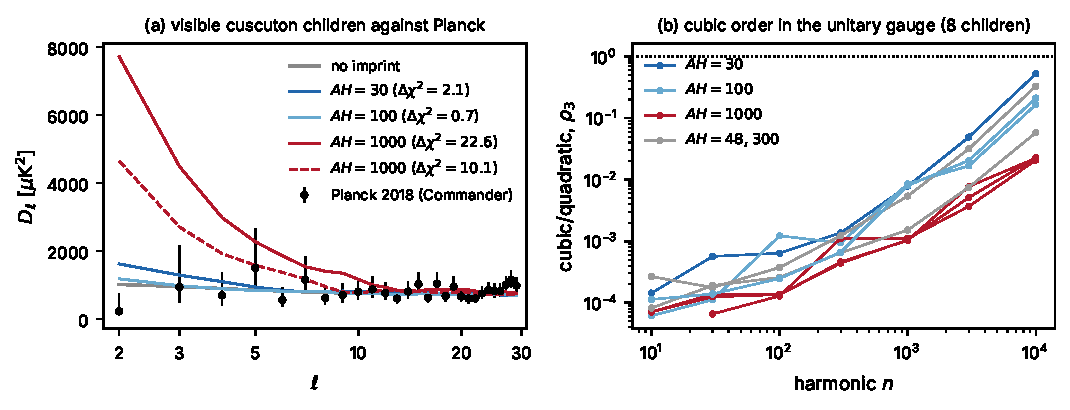
\includegraphics[width=\textwidth]{figures/fig_cuscuton.pdf}
\caption{The cuscuton birth. (a) Large-angle temperature spectrum of the visible children (the state A2, set in the contraction at $\Delta\ln a=2$ before the bounce window), with CLASS on a flat background, against the Planck 2018 spectrum; $\Delta\chi^2$ is relative to the same spectrum without the imprint. (b) Ratio of the cubic to the quadratic ADM Lagrangian in the unitary gauge, maximised over the history, against the harmonic $n$, in the eight children of the test (an informative reading of an inconclusive test).}
\label{fig:cuscuton}
\end{figure}

\paragraph{What the second realisation shows.}
The birth can be computed from a covariant action, with healthy linear scalars and tensors and tolerant to anisotropy; at cubic order, informative readings of inconclusive tests find it perturbative in the computed modes, which is evidence, not a proof of nonlinear stability. It is an alternative to the NPQT birth, not a replacement: it has no eternal branch, the parent bounces once and must be larger ($AH\ge30$) and carry a condensate of $\chi$, its past is singular, and the theory is an effective one with a preferred foliation, whose sign $\lambda<1$ may carry a non-perturbative instability in the ultraviolet~\cite{Afshordi2009}. The modes $n=0$ and $1$, loops and an ultraviolet completion are not computed; interactions between distinct modes have only been evaluated in exploratory calculations outside the released code, for a few triads of modes propagated through the bounce, as coefficients of the cubic action rather than as a bispectrum.
The two realisations feed the same inflationary attractor: near the pivot the cuscuton shifts $n_s$ by $1.7\times10^{-6}$ and $r$ by $+0.26\%$ relative to general relativity computed in the same way. Both realisations have negative $\Omega_K$ by construction. They share the dark-sector calculation under the adopted reheating and network histories. They differ where the bounce or the cuscuton act directly: the imprint at the largest scales and the late-time Newton constant, $G_{\rm cos}<G_N$.

\subsection{Pocket inflation and reheating}
\label{sec:pocket}

A region that rolls out of the eternal regime, or a direct child, inflates for its last $N_* = 51.6$ observable e-folds on the plateau attractor, giving
\begin{equation}
n_s = 0.9728,\qquad r = 0.0050,
\end{equation}
($+1.9\sigma$ from Planck 2018~\cite{Planck2018X}, $-0.4\sigma$ from ACT DR6~\cite{ACTDR6}, below the BICEP/Keck bound $r<0.036$~\cite{BK18}). These are the first-order slow-roll values that the chain computes; integrating the modes exactly (the general-relativity control of the test U58b) gives $n_s=0.9734$ and $r=0.0049$, $6.6\times10^{-4}$ higher in $n_s$ ($+2.0\sigma$ and $-0.3\sigma$) and $2.8\%$ lower in $r$, differences below current uncertainties.
For the adopted phenomenological reheating history, fixing $V_0$ from the amplitude fixes $n_s$ and $r$. With the cuscuton birth, relative to that exact control and computed in the same way, they move by $\Delta n_s=1.7\times10^{-6}$ and $\Delta r/r=+0.26\%$ (\S\ref{sec:cuscuton}).
Reheating is modelled with an effective friction (\S\ref{sec:open}) through a portal $\sigma\chi|H|^2$ that softly breaks the symmetry between the two sheets of the plateau, $\chi>0$ and $\chi<0$ (only $\chi>0$ hosts observers), with $T_{\rm rh}\approx2.3\times10^{9}$\,GeV and no dark radiation from reheating ($\Delta N_{\rm eff}\sim10^{-9}$).
The eternal regime requires $|V'/V| < 1.2\times10^{-6}$ per $\Mpl$ in the landing zone, $\chi\sim 5\times10^2$--$10^3\Mpl$; the undeformed pole plateau satisfies it (by a factor $\approx3$ at $\chi=10^3\Mpl$, and marginally at $\chi_{\rm et}$, where the bound defines the eternal regime), but any steeper deformation removes eternal children (\S\ref{sec:open}).

\subsection{Ordering of \texorpdfstring{$Q$}{Q}, strings, the decay constant and the Goldstone mass}
\label{sec:F}

During inflation $Q$ is held at the origin by $\xi_Q R S$; after inflation it orders into the $\RP$ vacuum, and ordering in causally disconnected patches leaves a network of $\Ztwo$ global strings, which radiates the three Goldstones.
The massive modes decay at tree level, much earlier than $\chi$.

The decay constant is $F=2f_a$.
An earlier stage of the chain fixed it at $F_0\simeq1.07\times10^{15}$\,GeV, the value that follows from the benchmark ordering scale $\mu/H_*=0.30$ of an earlier stage.
That stage only requires $\mu/H_*\le0.87$, and the CMB bound on global strings requires $F\le1.26\times10^{15}$\,GeV; we therefore treat $F$ as a free parameter with $F_0$ as its ceiling, and quote results as $F/F_0$.
The choice matters: at fixed abundance the Goldstone mass scales roughly as $m_G\propto F^{-4}$, and the benchmark is where the dark matter is hottest.
A smaller $F$ delays the ordering of $Q$: if the ordering scale is proportional to $F$, by $\tfrac12$--$\tfrac23\ln(F_0/F)$ e-folds depending on the equation of state, at most $\simeq1.9$ at the lower edge of the band. The network is then born somewhat later with the same correlation length in horizon units, and on the lattice it forgets its initial density within a few units of $\ell$ (\S\ref{sec:network}), so we expect no effect at $\ell\approx80$--$90$; this is an argument, not a computation. A smaller $F$ also lowers the $\ell$ of the collapse, from $\simeq94$ at $F_0$ to $\simeq80$ at the lower edge; the band rows scale the collapse yield linearly with their own $\ell$, and with the fitted exponent of \S\ref{sec:collapse} the soft momentum would be at most $6\%$ lower, so the band is slightly conservative there.

A small explicit breaking, $-\varepsilon Q_{11}=-\varepsilon n_1^2$, gives the Goldstones a mass $m_G$. Its domain-wall number is one by topology: on $S^3$ the term would have two minima, $n_1=\pm1$, but in $\RP$ they are the same point, and around a string, where the angle of $n$ winds by $\pi$, the potential has a single minimum.
The three Goldstones are exactly degenerate, protected by the ${\rm O}(3)$ that the breaking leaves intact, so the dark matter is an ${\rm O}(3)$ triplet: its fields are scalars, but in the non-relativistic limit three degenerate scalars obey under gravity the same equations as spin-1 wave dark matter, with the ${\rm O}(3)$ charge in the role of the spin~\cite{AdsheadLozanov2021,Amin2022VDM}. Its distinctive halo signatures, such as weaker interference granules, need masses below $\sim10^{-19}$\,eV and are out of reach in the band; its self-interaction is at most as strong as that of a single axion with the same $f_a$, so the superradiance edge of \S\ref{sec:band} is not weakened; and each field grows its own scalar cloud at the superradiance rate of a single axion of the same mass. Since the stress tensor is the ${\rm O}(3)$ singlet $\sum_a\partial\phi_a\partial\phi_a$, the annihilation power of a cloud with amplitudes $\psi_a$ goes as $|\psi\cdot\psi|^2$ instead of $|\psi|^4$, and for clouds grown from independent Gaussian seeds its average ratio is $2/(N_f+1)=1/2$ for $N_f=3$ fields, so the cloud would radiate on average $1/2$ of the gravitational-wave annihilation power of a single field. Because the dynamics conserves the ${\rm O}(3)$ charge and the graviton carries none, annihilation can only remove neutral pairs, and the identity $|\psi\cdot\psi|^2+\mathcal{Q}^2=|\psi|^4$ stops it when the number of quanta has fallen to the charge $\mathcal{Q}$; for clouds grown from random seeds, on average $2/3$ of such a cloud is locked by its charge and never annihilates, so the line is weaker, shuts off earlier and leaves a long-lived charged cloud (an estimate that ignores the charge that the black hole may absorb and that scalar waves emitted through the self-interaction may carry away).
It is added by hand: every term of the common action involving $Q$ is exactly ${\rm O}(4)$ invariant (verified numerically to $10^{-15}$) and the symmetry is not anomalous, so neither radiative corrections, nor the portal to $\chi$, nor instantons of the $Q$ sector generate a mass, and estimates of Planck-suppressed wormhole effects give $m_G\ll10^{-400}$\,eV.
Within the effective theory $\varepsilon$ is a bare parameter, and a technically natural one: setting it to zero restores ${\rm O}(4)$, so the loops of the model renormalise it only multiplicatively, and the mass is constant at all temperatures, as the lattice assumes. As for the axion, the danger is quantum gravity: Planck-suppressed operators that break the symmetry would give a much larger mass unless something forbids them up to dimension $n\approx20$--$26$. A gauged discrete symmetry acting on $Q$ alone cannot: every finite subgroup of ${\rm O}(4)$ already allows an ${\rm O}(4)$-breaking invariant of degree at most $6$ in $Q$ ($12$ if it contains reflections), and if $\varepsilon$ were the leading term such a symmetry allows, its minima would be degenerate, because a symmetry that forbids $-\varepsilon Q_{11}$ fixes no point of $\RP$ (at least $12$ vacua on $\RP$ in the cases we computed), and the network would leave stable domain walls (an exploratory calculation), the analogue of the quality--cosmology tension of the post-inflationary axion~\cite{LuReeceSun2023}. What would remain is an ${\rm O}(4)$ that is accidental, with $Q$ composite and the first breaking operator of dimension $20$--$26$, which by itself would give a mass in the band; the accidental symmetries of known chiral gauge theories are abelian and reach dimension $12$~\cite{ContinoPodoRevello2022}, and a non-abelian one is broken already at dimension six by products of its left and right currents, which induce $-\kappa\,{\rm Tr}(EQ)$ with a generic $E$ as photon exchange splits the pion masses (a spurion argument, checked algebraically), with $\kappa$ many orders of magnitude too large. A mass in the band therefore needs quantum gravity to break global symmetries only through exponentially suppressed effects, as estimated above, rather than through local operators with coefficients of order one; this is an assumption about quantum gravity, common to any ultralight pseudo-Goldstone of a non-abelian symmetry. The leading term of such a breaking is generically $-\kappa\,{\rm Tr}(EQ)$ with a non-degenerate $E$, which keeps $N_{\rm DW}=1$ but breaks the ${\rm O}(3)$. On the lattice ($192^3$), a non-degenerate breaking $-\kappa\,{\rm Tr}(EQ)$ with Goldstone masses in the ratio $1:\sqrt2:2$ leaves the soft quanta of the collapse $13\pm1\%$ slower than with the degenerate triplet, within the preregistered $\pm15\%$ (\textsc{igual}), and puts $59\%$ of them in the lightest Goldstone, against $39\%$ for independent species. We build no ultraviolet origin. A hidden sector that confines at $\Lambda_H\simeq(m_Gf_a)^{1/2}\approx2$--$56$\,keV is not a simple alternative: coupling $Q_{11}$ to heavy fermions charged under it regenerates the breaking at one loop, far above the required $\varepsilon$, so the coupling would have to be purely non-perturbative, and the hidden sector would have to be much colder than the visible one, since the walls form at visible temperatures of $\sim0.1$--$10$\,MeV, where it would still be deconfined.

The dark matter is the misaligned field, which starts oscillating at $H\sim m_G$, plus the Goldstones radiated by the network before it collapses, plus the soft Goldstones released when, at $H\simeq m_G/3$, walls attach to the strings and the string--wall network collapses (\S\ref{sec:collapse}).

%=====================================================================
\section{The \texorpdfstring{$\RP$}{RP3} string network on the lattice}
\label{sec:network}
%=====================================================================

The lattice comparison of the $\RP$ and U(1) networks is reported in full in a companion paper~\cite{rp3_paper}; we summarise what the dark sector uses.
Both models are evolved in the same C code in a radiation-dominated background, with physical cores, matched Goldstone decay constant and core mass ($m_r^2=0.24$ in code units), a symplectic leapfrog and $m_r a\,dx\le1$; strings are detected from the $\Ztwo$ holonomy (or the U(1) winding), $\xi=L\tau^2/(4V)$, and the free Goldstone radiation is measured with the kinetic estimator of Ref.~\cite{GHV2018}.
$\RP$ networks are measured at $576^3$ ($\ell_{\rm end}=5.66$) against U(1) at the same size; the U(1) control at $768^3$ passes preregistered scaling gates (initial-condition memory $7.6\%$).

\begin{itemize}
\item \textbf{Density.} The ratio is $\Rxi\simeq1.6$ for every protocol tested: sparse and dense starts, with and without draining the initial massive radiation, and networks started late and dense. At $\ell=5.61$ the declining late-dense and rising sparse networks give $\Rxi=1.57$ and $1.68$, respectively (Fig.~\ref{fig:bracket}).
\item \textbf{A systematic of the emission estimator.} The kinetic estimator counts conversion of the initial massive radiation into Goldstones as string emission. This contribution is $19\%$ ($\RP$) and $28\%$ (U(1)) of the measured emission for the sparse starts. For the dense U(1) start, the drain and a direct measurement of the radial-to-Goldstone transfer both put it above half. The exploratory dense $\RP$ comparison across resolutions suggests a similar share.
\item \textbf{Emission.} With the bath drained, $\RG=1.56\pm0.09\,({\rm stat})\pm0.08\,({\rm sampling})$, i.e.\ $\RG=1.56\pm0.12$. Preregistered tests bound the dependence on the drain (at most $1.9\pm1.4\%$), on the time step ($<2\%$ in $\RG$, $<1\%$ in $\Rxi$), on resolution and on volume; the snapshot-sampling systematic was adopted after the data. Per unit string length the $\RP$ network emits within $13\%$ of U(1) from both sides of the attractor.
\item \textbf{Spectrum.} The slope of the instantaneous emission at $\ell=5$ is $q=0.87\pm0.06$ with our estimator, but an independent re-implementation shows that the convention used to map the physical fitting window onto lattice momenta moves it to $0.89$--$0.90$, and a fit weighted by the spectrum gives $0.94\pm0.04$; we quote $q$ as compatible with $1$.
\end{itemize}
Without the collapse these numbers would decide survival. With the collapse included (\S\ref{sec:collapse}) the emission before the collapse is below $0.02\%$ of the dark matter, and the network enters the dark sector mainly through its energy at $H\simeq m_G/3$, i.e.\ through $\Rxi$ and the ratio of string energies, which we take equal to $\RG$ ($R_\rho=1.56$, a declared assumption).

\begin{figure}[t]
\centering
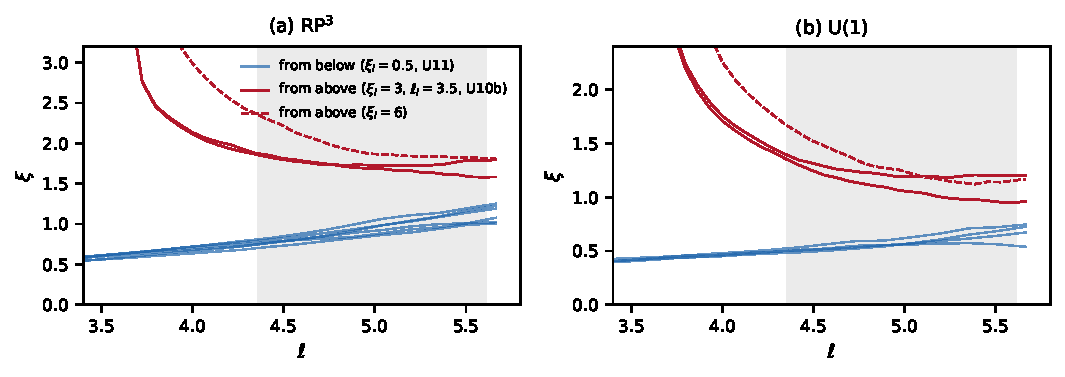
\includegraphics[width=\textwidth]{figures/fig_bracket.pdf}
\caption{The scaling attractor bracketed at $576^3$. Blue: drained networks starting sparse ($\xi_i=0.5$), approaching from below. Red: drained networks started late ($\ell_i=3.5$) and dense ($\xi_i=3$ solid, $6$ dashed), approaching from above. The shaded band is the analysis window.}
\label{fig:bracket}
\end{figure}

%=====================================================================
\section{The collapse of the string--wall network}
\label{sec:collapse}
%=====================================================================

\subsection{Why the collapse dominates}

When the walls appear, at $H=m_G/3$, the network energy density is $\rho_{\rm net}=4\xi\pi f_a^2\ell H^2$ and the misalignment energy is $\rho_{\rm mis}=\tfrac38m_G^2F^2$.
At the cosmological $\ell\simeq90$, $\rho_{\rm net}/\rho_{\rm mis}\simeq100$ for a network with constant density and up to $\sim2000$ if $\xi$ grows logarithmically.
If a fraction $\eta$ of that energy ends as Goldstones of mean energy $c\,m_G$, the collapse adds $K=(8\pi/27)\,\xi\ell\,\eta/c$ quanta per misalignment quantum.
A bracket $K\in\{0,1\}$, the natural guess before the inventory, does not hold: the inventory gives $K\sim3$--$800$ depending on $c/\eta$ and on the density branch, and the abundance condition
\begin{equation}
\big[\Omega_{\rm mis}(m_G)\,(1+K) + \Omega_{\rm em}(m_G)\big]\,h^2 = 0.12
\end{equation}
then lowers $m_G$ by two to four orders of magnitude with respect to an estimate with the string emission alone.
A classic U(1) simulation of the full string--wall system~\cite{Hiramatsu2012} finds a collapse contribution about ten times the misalignment, with mean energy $\simeq3.3\,m_a$ per axion and with all the network energy assumed to end in axions ($\eta=1$), i.e.\ $c/\eta\simeq3$, the warm end of our preregistered range.

Two consequences follow before any Lyman-$\alpha$ computation.
Branches in which the string density keeps growing up to $\ell\simeq90$ need the collapse to put almost all its energy into very hard quanta ($\eta\lesssim0.05$--$0.1$), which no simulation shows: they are disfavoured.
For a constant density (the branch supported by the largest U(1) simulations~\cite{Correia2025spectrum,Correia2024terasite}), what matters for Lyman-$\alpha$ is a single combination: with the population written as a soft part, the suppression depends only on $X=K\,\bar c\,r$, the soft momentum released per misalignment quantum, where $\bar c=\sqrt{c^2-1}$ is the mean momentum in units of $m_G$ and $r$ measures how late the collapse ends.
With the constant-density normalisation at $\ell\simeq90$ and $R_\rho=1.56$,
\begin{equation}
X = \frac{8\pi}{27}\,R_\rho\,\xi_*\ell\;Y \simeq 162\,Y ,
\end{equation}
where $Y$ is the soft yield per unit string energy; a U(1)-like collapse ($\eta=1$, $c=3$, $r=1$) has $Y=0.94$.

\subsection{The collapse measured on the lattice}

To measure $Y$ we evolve the $\RP$ field with the explicit breaking on $512^3$ lattices until the network has disappeared, with two protocols (sparse and dense string densities at the onset of the collapse, $\xi_1\approx0.7$ and $2.4$) and two seeds each, and count the Goldstone quanta of the final state; the counter reproduces the homogeneous equation to $\le1.6\%$, and each network must pass four validity checks (strings and walls gone, no site far from the vacuum, a flat count).
The soft momentum released, in units of $m_G a_1$ per misalignment quantum and with the misalignment population subtracted, is $X_{\rm lat}=\sum_{k<10m_Ga_1}k\,n_k/(m_Ga_1N_{\rm mis})$.
At $\ell_1\simeq4.3$ the preregistered verdict was a soft collapse, $Y=1.70\pm0.55$, but by the narrowest margin (the threshold was $Y-\sigma>1.14$ and the result $1.150$), and two reasonable analysis choices would move it to the intermediate class; we therefore do not lean on the label.
Three findings matter more than the label.
\begin{itemize}
\item \textbf{$\RP$ collapses like U(1).} At $512^3$, the same protocols with a U(1) field in the same code give $Y=1.58\pm0.50$; per protocol and seed the ratio is $1.06$--$1.08$. The $\RP$ network leaves more soft quanta only because it has more strings, and per quantum it is slightly softer (mean momentum $c_p\simeq4.3$ against $5.8$, in units of $m_G$ at the end of the collapse). Our U(1) does not reproduce the analytic U(1)-like collapse ($Y=0.94$); the lattice value is $1.7$ times larger, which may be a property of our small $\ell$ and short mass hierarchy.
\item \textbf{The soft momentum depends little on the string density.} Across protocols, $X_{\rm lat}$ changes by $15\%$ when the string density at the onset changes by a factor $5.5$; the extra energy of dense networks goes into hard quanta, which do not matter for Lyman-$\alpha$. We therefore decompose $X=X_0+y_s\,Z$, with $X_0$ the part independent of the string energy $Z$. A natural reading, not tested, is that the soft quanta come from the walls stretched across the horizon, whose area per Hubble volume is fixed at the horizon scale, while the extra string length of dense networks sits in sub-horizon loops that release hard quanta when the walls pull them in.
\item \textbf{It grows with $\ell$.} $X_0$ is larger at larger $\ell_1$, so the favourable reading in which the soft yield stays at its lattice value ($X\approx8$, cold even at $F_0$) is not supported. How fast it grows decides the band of $F$. Several things change together with $\ell_1$ between our lattices (the hierarchy between the horizon and the core, the epoch at which the collapse ends, the box size in Hubble units), and with these data the growth cannot be attributed to one of them.
\end{itemize}
The collapse ends late: the walls fall to $10\%$ at $a\simeq1.8\,a_1$ and the number of quanta settles at $a\simeq2.4\,a_1$.
The measured spectrum of the soft excess has a mean momentum $\bar x=5.83\,m_Ga_{\rm osc}$, hotter than the log-normal with $\bar x=3$ assumed before it was measured.

\subsection{Extrapolation to \texorpdfstring{$\ell\simeq90$}{ell ≈ 90}}

Two lattice sizes could not separate extrapolations that grow with $\ell$, and an independent re-analysis showed that our first reading overstated the evidence against a constant $X_0$.
We therefore repeated the protocol at fixed $\ell_G$ relative to $\ell_1$ on four lattice sizes, $256^3$, $384^3$, $512^3$ and $576^3$ ($\ell_1=3.61$, $4.01$, $4.30$, $4.42$; larger lattices fail the counter validation, by $5.4\%$ and $6.5\%$ against $5\%$).
With four networks per mass the masses scattered more than their errors and the exponent was undetermined; the preregistered remedy, twelve networks per mass with the same analysis, gave a smooth, monotonic $X_0(\ell_1)$ (Fig.~\ref{fig:collapse}a):
\begin{equation}
X_0 = 6.49\pm0.32,\ 7.50\pm0.43,\ 8.20\pm0.35,\ 8.57\pm0.42;\qquad X_0\propto\ell_1^{\,p},\ \ p=1.35\pm0.31 .
\end{equation}
The $576^3$ networks were run on a GPU with a JAX port of the kernel that reproduces the C code to machine precision on a control network.
The preregistered extrapolation, $\Xu=X_0(90)+162\max(y_s+2\sigma,0)$ with the least favourable string term ($49$), gives
\begin{equation}
\Xu \simeq 556\qquad (244\text{--}1367\ \text{for}\ p\pm\sigma_p),
\end{equation}
which the verdict logic classifies as undecided because the interval crosses the boundaries it was asked about.
The other models that fit the data give $\Xu\simeq218$ ($X_0\propto\ell_1$) and $273$ (linear in $\ell_1$); a constant $X_0$ ($\Xu\simeq56$) is disfavoured by $\Delta\chi^2\approx19$ (Fig.~\ref{fig:collapse}b).
The data cannot distinguish the three growing forms, because the extrapolation multiplies $\ell$ by more than twenty.
\emph{Informative reading.} In the sparse networks of the four lattice sizes the mean momentum per quantum at the end of the collapse is constant, $c_p\simeq3.49$--$3.55$, while the end of the collapse moves as $r_W\propto\ell_1^{0.53}$; this is the behaviour expected if the walls must first overcome a string tension that grows as $\ell$, which delays the collapse to $H\sim\sigma_w/\mu\propto m_G/\ell$ and gives $r\propto\ell^{1/2}$ in radiation domination, and nothing in this argument saturates at larger $\ell$.
If the network energy is frozen when the walls appear and released at the end of the collapse, the soft momentum grows as $\ell\,r\propto\ell^{3/2}$; if the network keeps scaling, and losing energy, while it waits, it grows as $\ell$.
The fitted exponent, $p=1.35\pm0.31$, lies between these two readings, so the physics does not select among the models that fit any more than the data do; the energy budget, $X\lesssim162\,r$, allows the central extrapolation if $r(90)\gtrsim3.4$, as the $\ell^{1/2}$ delay gives.
All of them give $\Xu>194$, the value below which the benchmark $F_0$ would have passed the Lyman-$\alpha$ screening (\S\ref{sec:band}).

\begin{figure}[t]
\centering
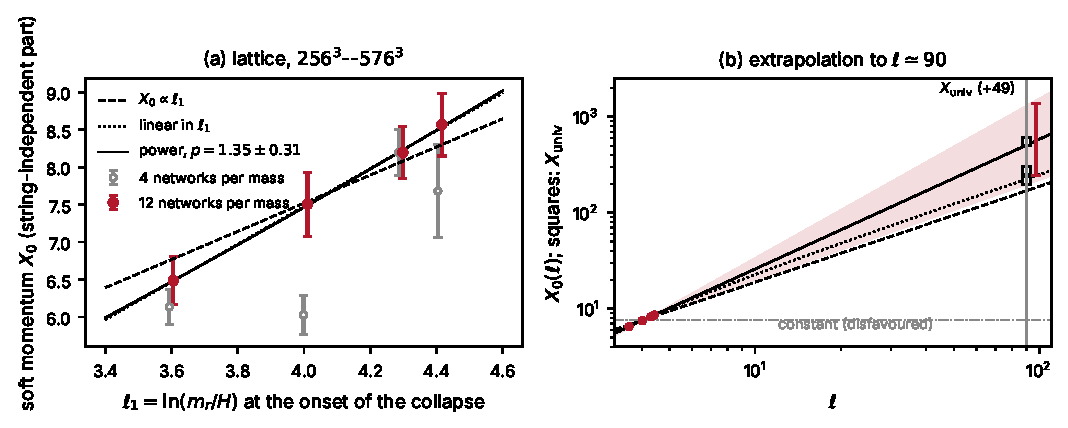
\includegraphics[width=\textwidth]{figures/fig_collapse.pdf}
\caption{The soft yield of the string--wall collapse. (a) String-independent soft momentum $X_0$ against $\ell_1$ at the onset of the collapse, with four (grey) and twelve (red) $\RP$ networks per lattice size, and the three growing models that fit. (b) Extrapolation of $X_0$ to the cosmological $\ell\simeq90$: power law with its $1\sigma$ band, $X_0\propto\ell_1$ (dashed), linear (dotted) and constant (dash-dotted, disfavoured). The squares are $\Xu$ for the three growing models, which include the string term ($+49$); the red bar is the preregistered interval.}
\label{fig:collapse}
\end{figure}

%=====================================================================
\section{Constraints and the band of \texorpdfstring{$F$}{F}}
\label{sec:band}
%=====================================================================

\subsection{Gates}

\paragraph{Lyman-$\alpha$ screening.}
The linear transfer function at $z=3$ is computed with CLASS v3.4.1~\cite{CLASSII,CLASSIV}, with the measured distribution read from a file as a non-cold species with the full Boltzmann hierarchy and an 18-line quadrature patch that places nodes uniformly in $\ln q$ (the fixed quadratures and the fluid approximation do not converge for these heavy-tailed distributions; the patched build is validated against analytic Fermi--Dirac and against our own synchronous-gauge solver).
The primary gate is a shape criterion: $T^2(k)$ on $0.5$--$20\,h$/Mpc is fitted with a grid of mixed cold plus thermal-warm models and must satisfy the mixed-dark-matter bound~\cite{GarciaGallego2025} or correspond to a thermal mass $\ge5.3$\,keV~\cite{Irsic2017}.
The area criterion $\dA$~\cite{Murgia2017} is reported with two references computed with the same set-up, strict ($0.234$, a 1\,keV mixed model at the bound) and wide ($0.336$, thermal 5.3\,keV); rows with $\dA$ above the wide reference that pass only the shape gate are marked ``by shape''.
Rows far colder than 5.3\,keV pass without CLASS.

\paragraph{Isocurvature.}
The collapse leaves white-noise isocurvature at scales $k_*\sim a H$ at the collapse, $f_{\rm iso}=C\,(k_{\rm CMB}/k_*)^3/A_s$, with $C=1$ and $k_*$ evaluated at the measured end of the collapse.
The gate is the Lyman-$\alpha$ bound $f_{\rm iso}<0.0084$~\cite{GarciaGallego2026}.
An earlier, self-made criterion was about 500 times stricter than the data and is superseded (appendix).

\paragraph{Black-hole superradiance.}
The primary gate is the $2\sigma$ excluded region from stellar black holes with self-interactions included~\cite{WitteMummery2025,BGLS2021}, with the effective decay constant between $F/4$ and $F$.
The bound from supermassive black holes~\cite{Unal2021,ChathirathasSchwetz2025}, which excludes $m_G<1.7\times10^{-17}$\,eV for our decay constants, rests on a single analysis that others consider less robust; we report it as a secondary bound.

\paragraph{Others.} $\Delta N_{\rm eff}\le0.3$ and the CMB bound on global strings; neither cuts in the band.

\subsection{The band}

With the measured population, the abundance solved for $m_G$ at each $F$, and the five gates, we computed families of rows at fixed $Y$ covering $\Xu$ from 160 to 1370 in two preregistered tests (84 rows through CLASS, the colder ones by the trivial-cold rule). Table~\ref{tab:band} and Fig.~\ref{fig:band} give the band.
In every family the upper edge is set by Lyman-$\alpha$; isocurvature fails only where Lyman-$\alpha$ already fails; the lower edge is set by stellar superradiance, and moves down as $\Xu$ grows because $m_G$ falls.
The dark matter is cold in the whole band and $96$--$99\%$ of it comes from the collapse.

\begin{table}[t]
\centering\small
\caption{Edges of the band of $F$ with the Lyman-$\alpha$ screening gates, against the soft momentum of the collapse in the universe. $^\dagger$: the edge row passes only by shape, with $\dA$ above the wide reference ($0.336$). The last column adds the secondary bound from supermassive black holes. The rows at $\Xu\simeq193$ and $\Xu\simeq320$ were tested with the full likelihood (\S\ref{sec:lyafull}).}
\label{tab:band}
\setlength{\tabcolsep}{4pt}
\begin{tabular}{rcccccc}
\toprule
$\Xu$ & upper edge & $\dA$ there & $m_G$ there (eV) & lower edge & $m_G$ there (eV) & with SMBH\\
\midrule
$\simeq160$--$193$ & $F_0$ & $0.335$--$0.378$$^\dagger$ & $6$--$8\times10^{-18}$ & $0.09F_0$ & $2\times10^{-13}$ & $0.7$--$0.85F_0$\\
$\simeq217$ & $0.85F_0$ & $0.328$ & $8.9\times10^{-18}$ & $0.09F_0$ & $1.3\times10^{-13}$ & $0.7F_0$\\
$\simeq272$ & $0.85F_0$ & $0.383$$^\dagger$ & $5.6\times10^{-18}$ & $0.09F_0$ & $8.4\times10^{-14}$ & $0.5F_0$\\
$\simeq315$ & $0.7F_0$ & $0.323$ & $9.4\times10^{-18}$ & $0.0625F_0$ & $2.8\times10^{-13}$ & $0.5F_0$\\
$\simeq396$ & $0.6F_0$ & $0.301$ & $1.1\times10^{-17}$ & $0.0625F_0$ & $1.8\times10^{-13}$ & $0.5F_0$\\
$\simeq477$ & $0.6F_0$ & $0.350$$^\dagger$ & $7.5\times10^{-18}$ & $0.0625F_0$ & $1.2\times10^{-13}$ & $0.5F_0$\\
$\simeq541$ & $\mathbf{0.5F_0}$ & $0.288$ & $1.3\times10^{-17}$ & $0.0625F_0$ & $9.2\times10^{-14}$ & $0.35F_0$\\
$\simeq674$ & $0.5F_0$ & $0.346$$^\dagger$ & $7.8\times10^{-18}$ & $0.045F_0$ & $2.3\times10^{-13}$ & $0.35F_0$\\
$\simeq859$ & $0.35F_0$ & $0.231$ & $2.3\times10^{-17}$ & $0.045F_0$ & $1.4\times10^{-13}$ & $0.35F_0$\\
$\simeq1333$ & $0.35F_0$ & $0.336$$^\dagger$ & $8.5\times10^{-18}$ & $0.03F_0$ & $3.1\times10^{-13}$ & $0.25F_0$\\
\bottomrule
\end{tabular}
\end{table}

\begin{figure}[t]
\centering
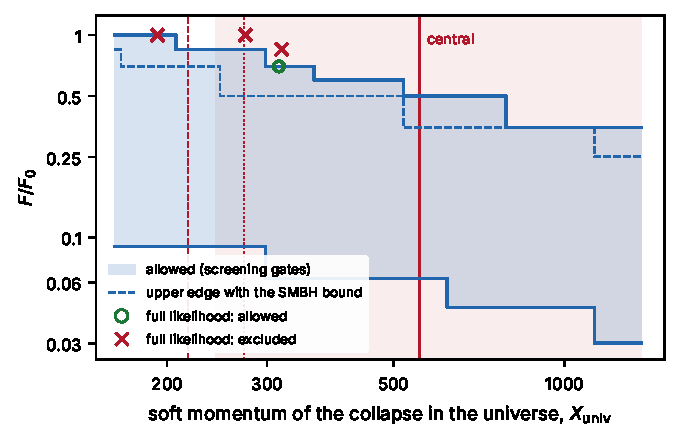
\includegraphics[width=0.72\textwidth]{figures/fig_band.pdf}
\caption{The band of $F$ against $\Xu$. Shaded: allowed by the Lyman-$\alpha$ screening, isocurvature, stellar superradiance, $\Delta N_{\rm eff}$ and CMB string gates; dashed: upper edge with the secondary supermassive black-hole bound. Vertical lines: the central extrapolation of the collapse (solid), $X_0\propto\ell_1$ (dashed) and linear (dotted); the light band is the preregistered interval. Markers: the four rows tested with the full Lyman-$\alpha$ likelihood.}
\label{fig:band}
\end{figure}

\subsection{The full Lyman-\texorpdfstring{$\alpha$}{alpha} likelihood}
\label{sec:lyafull}

The screening gates compare a transfer function with a family of thermal models at fixed cosmology.
We also ran the full likelihood of Ref.~\cite{Hooper2022}, with Planck 2018 (high-$\ell$ lite and low-$\ell$)~\cite{Planck2018V}, BAO~\cite{Alam2017} and the Lyman-$\alpha$ flux power spectrum, sampling the cosmological and intergalactic-medium parameters with MontePython~\cite{MontePython2019}.
Each case enters with a free amplitude $s$ of its non-cold component, $\omega_{\rm ncdm}=s\,f_{\rm nc}\,\Omega_{\rm DM}$ (so $s=0$ is cold dark matter and $s=1$ the model), with a flat prior on $[0,1/f_{\rm nc}]$ and $T^2(k;s)$ tabulated with CLASS.
A case is allowed if $p(s=1)/p_{\max}\ge e^{-2}$ with 30 bins, and undecided if the label changes with 20 or 45 bins or when one of the four chains is removed; the chains must reach $R-1<0.03$ in every parameter, also in halves.
The harness was validated with thermal mixtures, whose $95\%$ limits on the warm fraction, $0.27$ (1\,keV) and $0.42$ (2\,keV), fall inside the preregistered windows around the published fit.

The first two cases tested the band edges of an earlier stage with the log-normal population ($0.5F_0$ and $0.35F_0$): both pass with $p(s=1)/p_{\max}=0.87$ and $0.91$, but only because their suppression at $k=10\,h$/Mpc is below $0.15\%$, 50--100 times below what the data detect, so the posterior of $s$ is flat.
The decisive cases use the measured population at the upper edge (Fig.~\ref{fig:lyafull}):

\begin{table}[h]
\centering\small
\begin{tabular}{lcccccc}
\toprule
Case & $\Xu$ & $T^2(k{=}10\,h/{\rm Mpc})$ & $p(s{=}1)/p_{\max}$ & 20 / 45 bins & one chain removed & label\\
\midrule
$F_0$ & 193 & 0.972 & $0.111$ & $0.116$ / $0.126$ & $0.106$--$0.117$ & excluded\\
$F_0$ & 275 & 0.946 & $0.047$ & $0.045$ / $0.044$ & $0.038$--$0.057$ & excluded\\
$0.85F_0$ & 318 & 0.961 & $0.114$ & $0.112$ / $0.113$ & $0.110$--$0.120$ & excluded\\
$0.7F_0$ & 315 & 0.982 & $0.238$ & $0.239$ / $0.242$ & $0.225$--$0.246$ & allowed\\
\bottomrule
\end{tabular}
\end{table}

All four converged with four chains ($R-1\le0.017$, $\le0.026$ in halves; $\simeq1.8$--$2.0\times10^5$ points each) and no label changes with the binning or the jackknife.
The preregistered verdict is that the benchmark is excluded by the full likelihood and the $0.7F_0$ edge holds at $\Xu\simeq320$; the specification expected the benchmark to pass at $\Xu\simeq195$, on the basis of the calibration of the thermal validation, and that expectation failed.
The two exclusions at $0.11$ are close to the threshold ($-2\ln p=4.3$--$4.4$ against $4$), comparable to the bound on the error of evaluating $T^2$ at a fiducial cosmology ($|\Delta\ln L|\approx0.4$--$0.7$).
The posterior of $s$ is no longer flat: it decreases monotonically from $s\approx0$, so the data prefer cold dark matter to these rows, more strongly the larger the suppression.

\emph{Informative reading.} The row that passes has screening $\dA=0.323$ and the excluded ones $0.378$ and above, so the full likelihood cuts between $\dA\approx0.32$ and $0.38$; $\dA$ does not order the cases strictly (the rows with $0.378$ and $0.421$ give the same $p(s=1)/p_{\max}$), because the likelihood sees the full shape and redshift dependence.
The screening gate is therefore not conservative for rows that pass by shape only: the five rows marked so in Table~\ref{tab:band} become doubtful, and their edge may move down one step of the grid.
The central row ($\Xu\simeq541$, $0.5F_0$, $\dA=0.288$) is not affected.

\begin{figure}[!htbp]
\centering
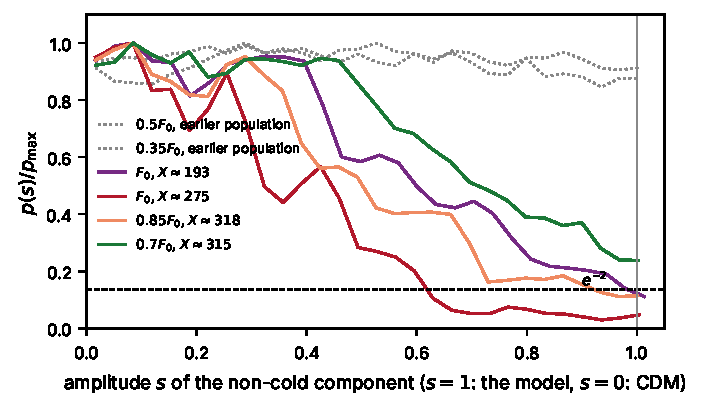
\includegraphics[width=0.72\textwidth]{figures/fig_lyafull.pdf}
\caption{Posterior of the amplitude $s$ of the non-cold component with the full Lyman-$\alpha$ likelihood (Planck + BAO + Lyman-$\alpha$, cosmology and intergalactic medium marginalised), normalised to its maximum. Dotted: two band edges with the earlier log-normal population, indistinguishable from cold dark matter. Solid: the measured population at the upper edge. The dashed line is the preregistered threshold $e^{-2}$ at $s=1$.}
\label{fig:lyafull}
\end{figure}

\subsection{Best estimate}

Combining the band with the extrapolation of the collapse:
\begin{itemize}
\item at the central extrapolation ($\Xu\simeq556$), $F\approx0.06$--$0.5F_0$, i.e.\ $f_a\approx0.3$--$2.7\times10^{14}$\,GeV and $m_G\approx1.3\times10^{-17}$--$9\times10^{-14}$\,eV, with the oscillation starting at $T\approx0.1$--$8$\,MeV; with the supermassive black-hole bound, $0.06$--$0.35F_0$;
\item over the whole preregistered interval of the collapse, $F\approx0.03$--$0.85F_0$, where $0.85F_0$ survives only near $\Xu\simeq220$ and with $\dA$ at the edge of what the full likelihood allows;
\item $F_0$, and with it the earlier benchmark, is excluded unless the soft yield grows more slowly than every model that fits: the full likelihood excludes it already at $\Xu\simeq193$, and the fitted models give $\Xu\ge218$. The two arguments are complementary, not independent: both assume a growing yield.
\end{itemize}

%=====================================================================
\Needspace{14\baselineskip}
\section{Predictions and falsifiers}
\label{sec:predictions}
%=====================================================================

Table~\ref{tab:predictions} lists the predictions and the measurements that could test them.

\begingroup
\small
\begin{longtable}{L{3.0cm}L{5.4cm}L{5.6cm}}
\caption{Predictions of the model and what would falsify them. The dark-sector entries assume the central extrapolation of the collapse unless stated.}
\label{tab:predictions}\\
\toprule
Observable & Prediction & Falsified or put under strain by\\
\midrule
\endfirsthead
\multicolumn{3}{l}{\tablename~\thetable\ continued}\\
\toprule
Observable & Prediction & Falsified or put under strain by\\
\midrule
\endhead
\midrule
\multicolumn{3}{r}{Continued on the next page}\\
\endfoot
\bottomrule
\endlastfoot
Scalar tilt & $n_s = 0.9728$ & $n_s$ outside $\sim0.965$--$0.98$ at $\sigma\lesssim0.002$\\
Tensor ratio & $r = 0.0050$ & $r<0.003$ (LiteBIRD, CMB-S4); $r\lesssim10^{-3}$ falsifies the pole plateau, and with it the inflation of the chain; with the cuscuton birth, $r$ is $0.26\%$ higher\\
Late-time $G$ & with the cuscuton birth only, $G_{\rm cos}/G_N=1/(1+\varepsilon_G)\approx0.996$ ($\lambda-1\approx-0.0026$) & a cosmological $G$ from the CMB and nucleosynthesis equal to the local one at the $0.1\%$ level would disfavour the cuscuton parameters, not the NPQT birth\\
Large-scale anomalies & none from the bounce: in the eternal branch, and in every direct child of the archived grid ($\gtrsim108$ e-folds; more than $300$ for the viable children of the radiation parent), the bounce lies far outside the observable universe; in a preregistered test over the births that can host our observable universe, it reaches $\ell\ge2$ with the curvature allowed by Planck for $3.8\times10^{-4}$ of them, and for none with the curvature of DESI DR2; with the cuscuton birth, its scale reaches $\ell\ge2$ in $5$ of $51$ hosts with Planck's curvature, with a quadrupole excess compatible with Planck in the tested cases $AH=30$ and $100$ ($\Delta\chi^2\le2.1$) & an imprint needs a parent with $AH\gtrsim1$--$3$ and a landing within $\lesssim0.02\,\Mpl$ of $\chi\approx4.1\,\Mpl$ (NPQT; its shape is not computed); with the cuscuton, a quadrupole $4.6$--$7.6$ times the reference ($AH=1000$) is disfavoured, and none explains the low quadrupole\\
Spatial curvature & closed, $\Omega_K<0$, with $|\Omega_K|<10^{-3}$ for $99.4\%$ of the births that can host our observable universe & a significant $\Omega_K>0$ (DESI DR2 with the CMB prefers it at $\approx2\sigma$) falsifies the birth in a closed parent, in both realisations, not the rest of the chain\\
Dark-matter nature & cold pseudo-Goldstones, $96$--$99\%$ from the string--wall collapse & a warm or hot dark-matter component detected in the small-scale power\\
Goldstone mass & $m_G\approx10^{-17}$--$10^{-13}$\,eV ($1.3\times10^{-17}$--$9\times10^{-14}$\,eV central) with $f_a\approx0.3$--$2.7\times10^{14}$\,GeV & superradiance or other ultralight-boson bounds closing this window at these decay constants\\
Small-scale power & suppression at most a few per cent at $k=10\,h$/Mpc near the upper edge ($T^2\approx0.98$ at the edge allowed by the full likelihood), vanishing towards the lower edge & a detected suppression larger than the upper edge allows is not produced by this sector; no detected suppression is consistent with lower $F$\\
Isocurvature & white noise at $k\gtrsim10^3$\,Mpc$^{-1}$, $f_{\rm iso}\approx5\times10^{-4}$ at the upper edge for the central $\Xu$ and up to $1.6\times10^{-3}$ over the interval ($C=1$), negligible towards the lower edge & a confirmed $f_{\rm iso}\approx0.006$ (the tentative Lyman-$\alpha$ detection~\cite{GarciaGallego2026}) fits only near $F_0$, which is excluded, unless $C\gg1$\\
Dark-matter multiplicity & an ${\rm O}(3)$ triplet of exactly degenerate Goldstones, if the ultraviolet origin of $m_G$ keeps the ${\rm O}(3)$; a breaking induced by quantum gravity need not keep it, and a non-degenerate one puts most of the soft dark matter in the lightest Goldstone (\S\ref{sec:F}); around black holes, superradiant clouds whose gravitational-wave annihilation line, at $2m_G/h\lesssim44$\,Hz, starts at $1/2$ of the power of a single axion on average (an estimate) and stops once the neutral part is gone, leaving $2/3$ of the cloud locked by its ${\rm O}(3)$ charge & an annihilation line that drains a whole cloud, as for a single axion, would disfavour the triplet, unless the charge leaks through the black hole or scalar emission\\
Dark radiation & $\Delta N_{\rm eff}\lesssim3\times10^{-3}$ & a detected $\Delta N_{\rm eff}\gtrsim0.05$ is not produced by this sector\\
Gravitational waves & global strings with $f_a\lesssim2.7\times10^{14}$\,GeV: below the LISA threshold~\cite{GHN2021} & a LISA global-string background (it would need $f_a\gtrsim5\times10^{14}$\,GeV)\\
Collapse at large $\ell$ & string-independent soft momentum $X_0$ fitted by $\ell_1^{1.35\pm0.31}$, $\Xu\simeq244$--$1370$ & a yield growing more slowly than $\ell_1$ (a constant one is disfavoured by $\Delta\chi^2\approx19$) would bring $F_0$ back below $\Xu\approx190$, where the full likelihood was not tested\\
Miniclusters & characteristic masses $\sim10^{-3}$--$10^{4}\,M_\odot$ across the band ($5\times10^3$ to $8\times10^{-3}\,M_\odot$ at the central $\Xu$), from the literature scaling $M\propto m_G^{-3/2}$; uncertain by about an order of magnitude & not computed as a population; a microlensing bound is not computed\\
\end{longtable}
\endgroup

For the adopted phenomenological reheating history, the inflationary predictions have no free parameter once $V_0$ is fixed.
The dark-sector ones are a band rather than a point because $F$ is free below its ceiling and the collapse is extrapolated over a factor of twenty in $\ell$.
Survival does not hinge on one side of the dispute about the large-$\ell$ behaviour of global-string radiation~\cite{GHV2021,Buschmann2022,KimParkSon2024,Saikawa2024,Benabou2025,Correia2025spectrum}: with the collapse dominating, the slope of that radiation is irrelevant, and a constant string density is still assumed because the growing branches need an implausibly hard collapse.
The band does not close at any $\Xu$ we tested: what would remove the dark sector is a combination of tighter superradiance bounds at the lower edge and tighter small-scale or isocurvature bounds at the upper edge.

%=====================================================================
\section{Open assumptions}
\label{sec:open}
%=====================================================================

\begin{description}
\item[Seed.] The small, closed, contracting patch is assumed, not derived. If its child enters the eternal regime it needs to exist only once; a direct child, the branch the coherence test favours, needs a seed of its own. It need not contain dust: a closed patch of pure radiation, with $\chi$ near its minimum, is a seed made of fields of the common action alone, and its coherent children come from tiny parents, $AH\le1$, that turn around close to the inflationary scale (\S\ref{sec:birth}). In the computed births of the dust model a parent is a closed dust ball a few plateau Hubble radii across ($AH\simeq0.4$--$21$), with $\chi$ at rest at its minimum except for a kinetic energy of $5\times10^{-11}$--$5\times10^{-2}$ of the dust, which the contraction pumps (\S\ref{sec:birth}). The velocity of $\chi$ is not a constraint: in the linear regime the bounce amplifies even a velocity of quantum size, and the patch takes an extra bounce if needed. What is not derived is where the patch comes from, and in the cases computed it does not form as a piece of an earlier, expanding era. For radiation, the core of an overdensity of the kind that forms primordial black holes is crossed by a shock before it bounces, in all $46$ preregistered configurations that form a horizon; when the core is made flat, its interior bounces before the shock arrives but out of step, and the past sound cone of every interior layer reaches the non-flat edge of the overdensity, so no part of the interior evolves as an isolated closed universe (an informative reading: the two preregistered tests of the flat core ended inconclusive on numerical validity). For dust, exploratory calculations that are not part of the released code find the same in another form: smooth overdensities do not rebound coherently, because their outer layers bounce later inside the core that has already re-expanded. A dust seed would need a closed patch dominated by pressureless matter and homogeneous up to a sharp edge, and no known mechanism gives these conditions together: an early era dominated by a modulus gives the matter but not the edge~\cite{KSW2015}, false vacuum trapped in a first-order transition gives the edge but not the matter~\cite{Liu2022PT}, and the pole plateau is too broad for the inflaton to fragment into oscillons~\cite{Amin2012}. The interior of a regular black hole in NPQT gravity does not provide the seed in this form either: a collapse that starts at low density reaches the bounce above the Planck density, and inside the horizon no core can stop and restart its collapse closer to the inflationary scale. A tiny closed universe of radiation therefore works as an initial state, not as a fragment of a larger universe; whether it is the first state or descends from one is open. The cuscuton birth needs a larger parent, $AH\ge30$, with an oscillating condensate of $\chi$, and its past is a big bang of general relativity (\S\ref{sec:cuscuton}); if its radiation carries vorticity, the contraction amplifies the vector potential by $(a_t/a_b)^2=8\times10^{3}$--$3.7\times10^{5}$, so the initial vorticity must be small, with a potential below $3\times10^{-7}$--$1.2\times10^{-5}$ depending on the parent. The seed is assumed there too.
\item[Field range.] Eternal inflation in the landing zone needs a plateau flat to $1.2\times10^{-6}$ per $\Mpl$ up to $\chi\sim10^3\Mpl$. We know of no UV construction that protects this; axion monodromy controls ranges of $\sim10\Mpl$, and the distance and de Sitter swampland conjectures~\cite{Obied2018} exclude it. The model lives outside the swampland or not at all. The shape of the plateau is a standard pole, which makes the required flatness stable against corrections analytic at the pole (\S\ref{sec:pocket}); what remains assumed is that the ultraviolet completion respects the pole over a geodesic range of $\sim10^3\Mpl$. The requirement belongs to the eternal branch: if our pocket is a direct, non-eternal child, the branch that the coherence of the parent's bounces favours (\S\ref{sec:birth}), the plateau needs to be flat only up to its landing value, $10$--$50\,\Mpl$ for at least $4.0\%$ of fertile births, still a super-Planckian range for the distance conjecture. With the parent of pure radiation the range is smaller: $4$ of the $17$ viable direct children have the field below $10\,\Mpl$ sixty e-folds after landing, the lowest at $7.0\,\Mpl$, so the plateau must be flat over about $7\,\Mpl$, twice the $3.6\,\Mpl$ of the observable e-folds and of the order of what plateau models such as Starobinsky inflation need. There the direct branch is no worse off than standard plateau inflation: its range is under tension with the distance conjecture but not excluded by it~\cite{ScalisiValenzuela2019}, while the refined de Sitter conjecture~\cite{OPSV2018}, with $|V'|/V\simeq0.025$ and $|V''|/V\simeq0.013$ at the pivot, and trans-Planckian censorship~\cite{BBLV2019} exclude it as they exclude any slow-roll inflation at this scale. A bounce within reach of the largest observable scales would need a landing below $\approx4.1\,\Mpl$, with at most $\approx60$ e-folds in total; the archived grid does not sample such births (its fertility criterion requires the field to exceed $5\,\Mpl$ after the bounce, which already gives $\approx108$ e-folds), and the imprint has not been computed. None of the viable radiation children comes close: the lowest still inflates more than $300$ e-folds after landing.
\item[Measure.] Only $\chi>0$ hosts observers: on the other sheet the portal $\sigma\chi|H|^2$ makes the Higgs tachyonic. The birth equations, which leave out the Higgs and its tiny portal, are symmetric under $\chi\to-\chi$ because the plateau is even, and the fractions of births quoted in this paper count both sheets; with a prior over parent states symmetric under $\chi\to-\chi$, exactly half of every class lands on $\chi>0$. The fraction of births that land in the eternal regime depends on the prior over parent states, not on a measure; weights within eternal inflation are measure-dependent, and so is whether observers live in pockets of the eternal branch or in direct children. Once eternal inflation is reached, volume favours the eternal branch, which the cuscuton birth does not have; the coherence of the parent's bounces favours direct children ($12.4$--$18.0\%$ of fertile births against $1.8$--$2.9\%$, \S\ref{sec:birth}). The predictions are not: every pocket and every direct child with more than $\sim60$ e-folds exits along the same single-field attractor, with the same $n_s$, $r$ and dark sector at a given $F$.
\item[Quantum backreaction at birth.] The contraction, bounce and kick are computed with a classical homogeneous $\chi$. Whether the quantum state of its zero mode, with its backreaction on $Q$, radiation and the NPQT background, follows the same history through the bounce and the launch is not established; a single mean background with fluctuating stress is itself an approximation near the bounce.
\item[Perturbations in NPQT.] Linear perturbations are not computed; standard perturbation theory on the NPQT background is assumed during inflation. At the bounce of the parent, where $\alpha\psi\to1$, the coherence test evolves spherical inhomogeneities nonlinearly with the NPQT equations (\S\ref{sec:birth}); non-spherical modes are not computed. During eternal and observable inflation $\alpha\psi=\alpha V_0/3\lesssim4\times10^{-4}$ for the viable children, so the background is that of general relativity to $\alpha^2\psi^2\lesssim2\times10^{-7}$; the CMB predictions rest on the theory reducing smoothly to general relativity at low curvature. Beyond spherical symmetry we know of no completion of the NPQT tower that we could use: a four-dimensional theory that reduces to it on homogeneous and spherical backgrounds and fixes the dynamics of shear and anisotropic curvature near saturation. Perturbative extensions explored separately (not part of the released code) stay healthy only for small anisotropies, and a closed form is not known. The non-spherical evolution of the parent through its bounce, the four-dimensional completion of the birth, is the step of the model we control least. The cuscuton birth (\S\ref{sec:cuscuton}) shows that a bounce with the same consequences can be computed from a covariant action, with healthy linear perturbations; it does not complete NPQT.
\item[Multi-bounce coherence.] Computed with an inhomogeneous $\chi$ for one bounce, in spherical symmetry and at one perturbation scale ($L\cdot H=1$), and extrapolated to several bounces by dividing the tolerated amplitude by their number, as in the dust model: the direct branch is viable and the eternal one marginal (\S\ref{sec:birth}). At the shorter scale $L\cdot H=0.3$ more than $20\%$ of the runs fail numerically, and the test is inconclusive there; in the dust model that scale leaves $2.2\%$ direct and $1.1\%$ eternal children. Two kinds of evidence, not part of the released code, suggest that this extrapolation is optimistic. Linear modes of $S^3$, evolved with our spherical solver through the bounces of three children of the radiation parent and checked against an independent linear calculation, show that the longest modes grow by large factors at every bounce, so the effect of a perturbation can compound from bounce to bounce instead of adding up. And an order-one perturbation localised far from the centre, which children that bounce once tolerate, focuses at its antipode and desynchronises the bounce of children that bounce twice. Neither became a verdict: the ten preregistered tests of children with several bounces (U46--U54) ended without a physical verdict, mostly on numerical validity. The children that bounce once do not rely on the extrapolation: $11.0$--$15.6\%$ of fertile births in the dust model with an inhomogeneous $\chi$ (against $12.4$--$18.0\%$ in all), and $4.3\%$ for the parent of pure radiation (against $10.5\%$). The viability of the direct branch rests on them.
\item[Anisotropy of the parent.] Computed for the parent of pure radiation as a Bianchi IX universe, with the NPQT acting on the matter and the shear left unregularised, where the viable direct children tolerate shape anisotropies far above $\zeta_0$ (\S\ref{sec:birth}). With the NPQT acting also on the shear, the other prescription that the reduced equations allow, it is not computed, and the verdict rests on a rule fixed after part of the production had been seen. The dust parent's anisotropy is not computed. With the cuscuton, which needs no prescription, all $52$ hosts tolerate anisotropies above $\zeta_0$ (\S\ref{sec:cuscuton}).
\item[Closing the loop.] Inflating islands seen from neighbouring pockets as black holes containing new eternal regions~\cite{GVZ2016}: an argument, without calculation. It is not needed for the model to exist: once reached, eternal inflation perpetuates itself. In a potential that decreases monotonically, as the pole plateau does, an eternally inflating region is separated from any pocket by a region that keeps rolling and inflating for a very long time, so it cannot appear as a black hole inside a pocket; that would need a wall or a barrier in the potential.
\item[Spatial curvature.] Every child is a closed FLRW universe, so the model predicts $\Omega_K<0$ (Table~\ref{tab:predictions}). Planck with lensing and BAO gives $\Omega_K=0.0007\pm0.0019$~\cite{Planck2018X}; DESI DR2 BAO with the CMB gives $\Omega_K=0.0023\pm0.0011$, a preference for an open universe at $\approx2\sigma$~\cite{DESI2025DR2,ChenZaldarriaga2025}. Almost every birth gives $|\Omega_K|$ far below either uncertainty, so the closed child is as disfavoured as flat $\Lambda$CDM; a significant $\Omega_K>0$ would falsify the birth in a closed parent. It would not touch the rest of the chain, which does not depend on how the pocket was born: an open universe from bubble nucleation~\cite{ColemanDeLuccia1980,BucherGoldhaberTurok1995} is the natural alternative birth, and it is not explored here. For the NPQT birth, in a preregistered test with the background alone, the inflation that makes the curvature of a closed child compatible with Planck pushes the memory of its bounce out of the observable sky in all but $3.8\times10^{-4}$ of the births that can host us; with the DESI DR2 curvature, in all of them (an informative reading). This is a statement about scales: the shape of a possible imprint is not computed. The cuscuton bounce keeps a longer memory, and its imprint and its comparison with Planck are in \S\ref{sec:cuscuton}.
\item[Late-time acceleration.] The cosmological constant of the late universe is taken from observation; the model does not explain it. The pole plateau ends at $V=0$, the NPQT corrections are negligible today, and a frozen Goldstone of this sector stores at most $\sim H_0^2f_a^2$, about eight orders of magnitude below the dark energy for $f_a$ in the band.
\item[The cuscuton as an effective theory.] The cuscuton birth uses an effective theory with a preferred foliation, whose sign $\lambda<1$ may carry a non-perturbative instability in the ultraviolet~\cite{Afshordi2009}. Its linear scalars, tensors and anisotropy are computed; the modes $n=0$ and $1$ and loops are not, interactions between distinct modes only in exploratory calculations, and its cubic order rests on informative readings of three inconclusive tests. The exit is hot by necessity, and with the effective friction of the chain it is hot by more than $42$ orders of magnitude in the branch condition (\S\ref{sec:cuscuton}); what is not computed is the microscopic reheating behind that friction. With a cosmological constant the branch would end in the future, no sooner than $11$ e-folds from today (an analytic extrapolation). The scale of its potential, $|U(0)|\approx1.4\times10^{5}V_0$, is not explained.
\item[$m_G$.] A bare, technically natural parameter of the effective theory; no ultraviolet origin is built. Planck-suppressed breaking must be forbidden up to dimension $20$--$26$, which neither a discrete symmetry acting on $Q$ alone nor an accidental non-abelian symmetry can do (\S\ref{sec:F}); the model therefore assumes that quantum gravity breaks global symmetries only through exponentially suppressed effects, and then $\varepsilon$ is a bare parameter. A breaking of that kind need not keep the ${\rm O}(3)$ of the triplet. The exact ${\rm O}(3)$ is therefore part of this assumption; a non-degenerate breaking has been tested only on the lattice, with masses in the ratio $1:\sqrt2:2$.
\item[$F$ and the ordering of $Q$.] $F$ is free below $F_0$; the delayed ordering at small $F$ (at most $\simeq2$ e-folds) is argued, not computed, to leave the network at $\ell\approx80$--$90$ unchanged (\S\ref{sec:F}).
\item[The collapse at $\ell\approx90$.] The soft yield is measured at $\ell_1\le4.42$ and extrapolated to $\ell\simeq90$; three growing forms fit equally well and give $\Xu$ from 218 to 556, with a preregistered interval up to 1370. The energy ratio $R_\rho$ of $\RP$ to U(1) strings is taken equal to the emission ratio; it enters only the string term of $\Xu$ ($49$ of the central $556$), because $X_0$ is measured on the $\RP$ lattice itself. Our lattice U(1) collapse is softer than the analytic U(1)-like one by a factor $1.7$ in $Y$; if the lattice overestimates $Y$ in both models, the band would move up.
\item[Isocurvature normalisation.] $C=1$ is not computed; with $C\gg1$ isocurvature would cut the upper edge. Our collapse lattices cannot measure it: at the end of the collapse they span only about one and a half Hubble volumes, so the white-noise plateau at $k\ll aH$ is outside the box, and the stored results keep the Goldstone number spectrum, not the density field. Measuring $C$ needs boxes many Hubble volumes across at the end of the collapse.
\item[Superradiance.] The stellar region is a digitised figure ($\pm0.1$\,dex); the supermassive bound rests on one analysis.
\item[Full likelihood beyond $\Xu\simeq320$.] At $\Xu\simeq272$ and $477$--$1333$, the rows that pass the screening by shape only have yet to be tested with the full likelihood. We evaluate $T^2$ at a fiducial cosmology. With $f_{\rm nc}\simeq0.98$ the model lies near the edge of the simulations behind the likelihood, although none of its internal range checks was triggered in any chain.
\item[Reheating bath.] Reheating uses an effective friction; the bath model and preheating are not computed.
\item[Network before radiation domination.] $Q$ orders shortly after inflation, while the oscillating inflaton still dominates, and with the effective friction the universe becomes radiation-dominated only at reheating, many e-folds later. The lattice networks are evolved in a radiation-dominated background (\S\ref{sec:network}). That the network has reached the radiation-era scaling state by the collapse at $\ell\approx80$--$90$, forgetting the earlier era and how it was born from the inflationary state of $Q$, is not computed at those scales; it rests on the attractor behaviour of \S\ref{sec:network}, measured only for synthetic initial conditions and at the small values of $\ell$ that the lattice reaches. A lattice test at $192^3$ gives a warning: a network already in the $\RP$ vacuum that spends part of its life in a matter-dominated era, with $\xi_QR$ acting, reaches the radiation era diluted, with $35$--$50\%$ fewer strings than a radiation-era network at $\ell=4.1$ (\textsc{recuerda}). The deficit closes on a scale of $\approx3$--$4$ units of $\ell$, so the $57$--$66$ units of $\ell$ in radiation before the collapse would erase it if that rate holds, which is an extrapolation. Ordering from the symmetric phase itself was not reached in that test: the tachyon at the ${\rm O}(4)$-symmetric point is weak ($m^2=-0.019$ against $m_r^2=0.24$), and from a small seed $Q$ ordered only at the end of the box (\textsc{inconcluso}). Two things bound the consequence. With the effective friction the network spends about $14$ e-folds in the inflaton era and then $57$--$66$ units of $\ell$ in radiation domination before the collapse. And the soft momentum of the collapse depends little on the string density (\S\ref{sec:collapse}), while the band is tabulated over the whole preregistered interval of $\Xu$: a memory of the birth would move the band outside the quoted one only if it changed the string-independent part of the yield by more than a factor of $2.3$, while a deficit of $50\%$ in the string density moves $\Xu$ by $\approx4\%$, through its string term.
\end{description}

%=====================================================================
\Needspace{8\baselineskip}
\section{Earlier models and discarded mechanisms}
\label{sec:history}
%=====================================================================

Four earlier models explored variants of the $\RP$ string network, pseudo-Goldstone dark matter and the hierarchical plateau. Preregistered tests led us to replace their birth mechanism. Local collapses within an expanding parent failed the coherence test. Sharp edges supported by tension fell faster than dust, and a core--envelope pair failed to generate the two centres required by the $1/\chi$ plateau. The tested inflated parents failed to produce new seeds, and production from scars or bubbles fell short by more than $4\times10^3$ in energy.

The dark sector was then tested in stages.
The first closure found a narrow conditional window if the network emitted at most $0.1$--$6\%$ of a U(1) network; the first lattice measurement gave an emission ratio far above that, so the closure with the measured efficiency failed in its original form, and the warmth gate was replaced by a Boltzmann transfer and Lyman-$\alpha$ gates.
The energy inventory ruled out the original bracket $K_{\rm sw}\in\{0,1\}$. We evolved the collapse population with CLASS, established the upper bound $F_0$, and replaced provisional isocurvature and superradiance criteria with observational bounds.
Successive lattice campaigns measured the collapse at one, two and then four masses, ultimately with twelve networks per mass. Each extrapolation updated the band, and the full Lyman-$\alpha$ likelihood tested its upper edge.
Appendix~\ref{app:log} lists every test.

%=====================================================================
\section{Reproducibility}
\label{sec:repro}
%=====================================================================

The repository~\cite{whalefall_chain}, a one-way export of the working repository with the source commit and the SHA-256 of every file, contains the chain, the coherence codes of the birth (with the original code of the dust model and every run with an inhomogeneous $\chi$), the lattice code with every collapse network and the summary of each emission test (the emission networks one by one are in the repository of the companion paper~\cite{rp3_paper}, \url{https://github.com/indigenica/whalefall-rp3-string-networks}), the CLASS patch and Lyman-$\alpha$ pipelines, the full-likelihood harness, the common-action symbolic checks, frozen inputs from earlier campaigns with SHA-256 provenance, every preregistration with its amendments and the report of each test up to U28, and the scripts that produce the figures of this paper from result files only.
For the parent of pure radiation (tests U33--U43 and the audit of U36) it contains the result files that the numbers check of this text reads, and the count of children that bounce once (\texttt{chain/u28\_un\_rebote.py}); for the tests U44--U56 it contains only the two result files of U55b that the numbers check reads; their codes, preregistrations and reports are in the working repository and are available from the author on request. For the cuscuton birth (tests U57--U66) it contains the codes, preregistrations, reports and result files, and the Planck 2018 spectrum that U62e reads; the intermediate rows of the long runs stay in the working repository. For the network before radiation domination and the non-degenerate breaking (U67, U68) it contains the lattice codes, the two kernel switches they add (off by default, with which the kernel is bit-identical to the production one), the preregistrations, reports and every network.
\begin{itemize}
\item The coherence tests of the birth run on one core of the cloud machine: that of direct children in $\sim4$\,min, and the $780$ runs of the parent with an inhomogeneous $\chi$ in $\sim3$\,h.
\item \texttt{make test} ($\sim3$\,min) and \texttt{make chain} ($\sim4$\,min) reproduce the chain and the contract on a laptop; the chain runs with the pole plateau by default and with the ten-level hierarchy on request.
\item Lattice runs used a 44-thread workstation, a 4-core cloud machine and, for the largest collapse networks, an A100 GPU with a JAX port of the kernel; the collapse networks took 0.4--2.6\,h each on the cloud machine and the GPU and 9--11\,h each at $512^3$ on the workstation, and each $\RP$ emission network at $576^3$ 1.5--2\,h.
\item CLASS v3.4.1 (commit \texttt{814ce59}) with the patch, which the environment check and the latest CLASS scripts verify before running. The full-likelihood chains (MontePython with Planck lite, BAO and Lyman-$\alpha$) took several days per campaign on the workstation; they are kept by the author and their summaries are in the repository.
\end{itemize}

%=====================================================================
\section*{Acknowledgments}
%=====================================================================

The author thanks the developers of CLASS and MontePython for making their codes public.

Most of the code, the preregistration documents, the audits and the revisions of this text were produced in an iterative workflow with an AI assistant (Claude Opus 5.5, Anthropic), under the direction of the author, who chose the scientific questions, the model ingredients, the tests and which results to accept.
The audits and critical reviews used separate AI sessions. GPT-6.1 Sol (OpenAI) contributed to the scientific review of the cuscuton branch and the editorial and reproducibility checks.
The author takes full responsibility for the content.

This research received no external funding, and none is currently in place; support to continue it would be welcome.

\appendix
%=====================================================================
\section{Test log}
\label{app:log}
%=====================================================================

Verdict labels are kept in the original (Spanish) form used in the specifications and result files; the internal codes index the repository.
Tests up to U15 that still bear on the model are listed; the others are in the index of preregistrations of the repository~\cite{whalefall_chain}.

\begin{small}
\begin{longtable}{L{1.3cm}L{6.0cm}L{7.0cm}}
\toprule
Test & Question & Preregistered verdict (and later reading)\\
\midrule
\endfirsthead
\toprule
Test & Question & Preregistered verdict (and later reading)\\
\midrule
\endhead
\bottomrule
\endfoot
U11 & Emission with the initial bath drained ($576^3$) & \textsc{limpia\_zona\_permitida} ($\RG=1.56\pm0.09$); \textsc{q\_menor\_que\_1} (later: convention dependent, $q$ compatible with 1) \\
U10b & Late dense starts, approach from above & \textsc{atractor\_acotado}, $\Rxi\in[1.57,1.68]$ \\
U13 & $m_G$ from the common action & \textsc{m\_g\_requiere\_ruptura\_nueva} \\
U15 & Lyman-ABGD likelihood at fixed cosmology & \textsc{inconcluso} (harness failed its validation) \\
U16 & Resolution and volume of the network ratios & \textsc{resolucion\_robusta} ($\Rxi$, $\RG$); volume: \textsc{volumen\_robusto} ($\RG$), \textsc{indeterminado} ($\Rxi$, no power) \\
U18 & Resolution with dense snapshots & \textsc{indeterminado}; snapshot-sampling systematic of $\pm5\%$ adopted after the data \\
U24 & Dependence of $\RG$ on the drain & \textsc{drenaje\_robusto} (at most $1.9\pm1.4\%$) \\
U25 & Time step of the production runs & \textsc{paso\_robusto} \\
U17 & Network energy at the collapse & \textsc{k\_sw\_fuera\_del\_rango\_tibia}: $K\sim3$--$770$, not $0$--$1$ \\
U17b & Collapse population through CLASS & \textsc{solo\_xi\_constante\_vive} \\
U17c & Critical collapse fraction for growing density & \textsc{rama\_comoda\_forzada} ($\eta_{\rm crit}\simeq0.1$; 0.05 for $\xi\propto\ell$) \\
U17d & Corrected balance with $R_\rho=1.56$ & \textsc{rama\_viva\_con\_colapso\_tipo\_u1} (passes by shape only; expectation failed) \\
U21 & Band of $F$ & \textsc{banda\_bajo\_el\_benchmark} ($F\le0.7F_0$; the benchmark fails) \\
U20 & Own isocurvature estimate & \textsc{isocurvatura\_recorta\_banda} (later: criterion $\sim500\times$ stricter than the data; superseded by U20b) \\
U22 & Pole plateau & \textsc{polo\_cambia\_nacimiento} (later: a counting error; corrected by U22b) \\
U22b & Birth statistics with the pole, full grid & \textsc{nacimiento\_robusto} ($R=0.94$) \\
U26 & Pole plateau adopted in the chain & \textsc{polo\_adoptado} \\
U19 & First collapse test ($320^3$) & \textsc{indeterminado} (counter not valid at that size) \\
U19b & Collapse of $\RP$ measured ($512^3$, 4 networks; U(1) control and a second mass) & \textsc{colapso\_blando}, by a margin of $0.01$ (later: fragile; $\RP\simeq$ U(1) per string energy; soft momentum depends little on $\xi$ and grows with $\ell$) \\
U17e & Measured population through CLASS & \textsc{banda\_recortada} \\
U23 & Superradiance with self-interactions & \textsc{superradiancia\_parte\_la\_banda} (stellar BHs set the lower edge) \\
U20b & Isocurvature with observational bounds & \textsc{isocurvatura\_no\_limita} \\
U17f & Upper edge over $\Xu\approx170$--$320$ & \textsc{borde\_0.7\_confirmado}; $F_0$ permitted for $\Xu\le194$, by shape (later: excluded by U15d) \\
U15b & Full Lyman-$\alpha$ likelihood: validation & \textsc{detenido} (physical rows stopped when superseded); validation passed ($f_{95}=0.27$, $0.42$) \\
U15c & Full likelihood at the earlier band edges & \textsc{rama\_viva\_permitida\_lya\_completo} (indistinguishable from CDM) \\
U19c & Collapse at four lattice sizes, 4 networks each & \textsc{indeterminado} ($\sigma_p=0.76$) \\
U19d & Same with 12 networks per size & \textsc{x\_univ\_indeciso} ($\Xu=244$--$1367$; $p=1.35\pm0.31$) \\
U17g & Upper edge over $\Xu\approx400$--$1370$ & \textsc{borde\_baja\_a\_0.35} ($0.5F_0$ at the central $\Xu$) \\
U15d & Full likelihood at the upper edge & \textsc{f0\_excluido\_lya\_completo}; \textsc{borde\_0.7\_sostenido} \\
U27 & Coherence of direct (non-eternal) children with the pole plateau, dust model & \textsc{rama\_directa\_viable}; \textsc{banda\_10\_50\_poblada} ($14.9\%$ direct, $3.6\%$ eternal, $4.9\%$ direct at $10$--$50\,\Mpl$) \\
U28 & Coherence of the parent's bounces with an inhomogeneous $\chi$ & \textsc{igual} in both classes; direct branch \textsc{viable} ($12.4$--$18.0\%$), eternal \textsc{marginal} ($1.8$--$2.9\%$); the preregistered solver could not cover the patch and was replaced before production \\
U33 & Parent of pure radiation: (A) fertile children below the Planck density; (B) coherence of its bounces & (A) \textsc{radiacion\_fertil} ($64$ children); (B) \textsc{inconcluso} (no solver passed all its gates) \\
U34 & Same as U33-B with a solver stable at maximum expansion & \textsc{inconcluso} (the filter fails its dust-limit gate) \\
U35 & Same with a filter that keeps homogeneity & \textsc{inconcluso} (same gate; production not run) \\
U36 & Same in linear theory & \textsc{inconcluso} (spectral convergence) \\
Audit U36 & Independent re-implementation of U36 & Gates passed; agrees child by child; \textsc{semilla\_radiacion\_viable} (direct branch, $10.5\%$; eternal inconclusive) \\
U37 & Anisotropy of the radiation parent (Bianchi IX) & \textsc{anisotropia\_inocua} with an amendment fixed after part of the production; \textsc{inconcluso} with the earlier rule \\
U38 & Radiation overdensity of primordial-black-hole type as a parent & \textsc{inconcluso} (invalid runs) \\
U39 & Same with a solver that crosses the neck & \textsc{inconcluso} \\
U40 & Does a shock reach the core before it bounces? & \textsc{padre\_caliente\_no\_coherente} (in all $46$ configurations that form a horizon) \\
U41 & Flat core: does the interior bounce coherently? & \textsc{inconcluso} (the interior bounces before the shock arrives, but out of step) \\
U42 & Causal domain of the interior bounces & \textsc{inconcluso} (global constraints above threshold); informative: the desynchronisation comes from the non-flat edge \\
U43 & Does the radiation birth depend on how NPQT approaches its saturation? & \textsc{inconcluso} (a regression gate on births without a child); informative: the same $64$ children with both alternatives \\
U44 & A radiation parent joined by a neck to a flat exterior & \textsc{inconcluso} (such parents cannot be built with small necks; large necks form trapped regions) \\
U45 & An order-one perturbation localised at the antipode of the parent & \textsc{cicatriz\_tolerada} (children that bounce once; children with several bounces not judged) \\
U46 & Same, children with several bounces & \textsc{inconcluso} (momentum constraint) \\
U47 & Same, with an absolute momentum constraint & \textsc{inconcluso} (by $0.1\%$ in a regression gate) \\
U48 & Same, with radial dynamics of $\chi$ & \textsc{inconcluso} (bounce counter near the centre) \\
U49 & Same, with a robust counter and localised validity & \textsc{inconcluso}; informative: a perturbation of width $0.2$\,rad desynchronises children that bounce twice \\
U50 & Linear modes of $S^3$ in the solver against an independent linear calculation & \textsc{inconcluso}; informative: agreement to $\le6\times10^{-3}$ for $n=2$--$6$, and the longest modes grow strongly at each bounce \\
U51, U51b & A conservative discretisation of the equatorial band & \textsc{inconcluso} (time-step gates) \\
U52 & The equatorial mode that violates the constraints & \textsc{inconcluso}; informative: imposing the mass constraint removes it \\
U53 & Linear modes through three bounces with the mass constraint imposed & \textsc{receta\_no} (the longest mode is not resolved in double precision); informative: $n=5$--$20$ reproduced to $\le0.73\%$ \\
U54 & U49 with the mass constraint imposed & \textsc{inconcluso} (no row passes validity and convergence) \\
U55 & The bounce imprint on the sky, from the background (which births would show their bounce at $\ell\ge2$?) & \textsc{inconcluso} (a badly chosen gate on the count of e-folds); informative: the curvature bound and the visibility at $\ell=2$ coincide within one e-fold \\
U55b & Same, with new data and an independent integrator & \textsc{huella\_rara} ($3.8\times10^{-4}$ of the hosts); none with the DESI DR2 curvature (informative) \\
U56 & Memory of the bounce in the visible modes (linear, scalar) & \textsc{inconcluso} (all four gates); informative: erased for modes above $2.5$ times the memory scale of the bounce \\
U57 & Birth with Einstein gravity and a cuscuton (background) & \textsc{inconcluso} (a constraint rule too strict for parents that do not inflate; two children at the edge of the branch) \\
U57b & Same, with new data and two rules amended after U57 & \textsc{cuscuton\_fertil} (children for $AH\ge30$) \\
U58 & Inflation with the cuscuton, parameters of an exploratory run & \textsc{inconcluso}; informative: that set changes the cosmological $G$ by $4.9\%$ and is excluded \\
U58b & Same, with the adopted parameters & \textsc{cuscuton\_compatible} ($\Delta n_s=1.7\times10^{-6}$, $\Delta r/r=+0.26\%$) \\
U59 & Linear scalars through the cuscuton bounce & \textsc{inconcluso} (a quadrature threshold below rounding; a two-point rule) \\
U59b & Same, with new data and rules chosen after U59 & \textsc{escalares\_sanos} \\
U60 & Anisotropy of the cuscuton parent (Bianchi IX) & \textsc{anisotropia\_inocua} \\
U61 & Curvature and imprint with the cuscuton children & \textsc{inconcluso} (constraint projection missing) \\
U61b & Same, with the constraint projected & \textsc{huella\_posible} ($5$ of $51$ hosts, $13\%$ with equal weight per parent size, with Planck's curvature; none with DESI DR2) \\
U62 & Bogoliubov coefficients through the cuscuton bounce & \textsc{rebote\_excita}, without physical reading (vacuum in an unphysical frame) \\
U62b & Same, in the physical frame & \textsc{inconcluso} (one numerical point); informative: the memory decays above a few $n_{\rm mem}$ \\
U62c & Primordial spectrum of the visible children & \textsc{inconcluso} (constraint lost in the backward contraction) \\
U62d & Same, from the parent's turnaround, projected to $C_\ell$ & \textsc{inconcluso} (sampling of one state) \\
U62e & Full $C_\ell$ with CLASS against Planck 2018 ($\ell=2$--$29$) & \textsc{mixto} (compatible for $AH=30$, $100$; disfavoured for $AH=1000$) \\
U63 & Cubic order near $\dot\varphi\to0$ & \textsc{inconcluso} (cancellations beyond double precision in the uniform-radiation gauge) \\
U63b & Strong coupling in unitary-gauge variables & \textsc{inconcluso} (a precision floor at $n=3\times10^4$); informative: no indication of strong coupling in the tested modes as $\dot\varphi\to0$ \\
U64 & Full cubic order in the unitary gauge & \textsc{inconcluso} (two gates missed narrowly); informative: cubic below quadratic in every computed mode \\
U65 & Tensors and vectors through the cuscuton bounce & \textsc{tensores\_con\_rasgos} (features of the size of the scalar ones; no vectors in the action) \\
U66 & Hot exit of the cuscuton children with the effective friction & \textsc{inconcluso} (a regression gate too strict for a sampled maximum); informative: all children exit hot \\
U66b & Same, with the friction varied by a factor of ten each way & \textsc{salida\_caliente} (margin $\ge10^{42.5}$) \\
U67 & $\RP$ network ordered by $\xi_QR$ in a matter era, then radiation ($192^3$) & \textsc{inconcluso} ($Q$ does not order in time from a small seed; weak tachyon at the symmetric point) \\
U67b & An ordered network through a matter era & \textsc{recuerda} ($35$--$50\%$ fewer strings at $\ell=4.1$, closing over $\approx3$--$4$ units of $\ell$) \\
U68 & Collapse with a non-degenerate triplet, $-\kappa\,{\rm Tr}(EQ)$ ($192^3$) & \textsc{inconcluso} (a mass gate, before any network) \\
U68b & Same, with the mass gate against the exact Hessian & \textsc{igual} (soft quanta $13\pm1\%$ slower; $59\%$ in the lightest Goldstone); a counter bug found by an external review was fixed and the networks rerun \\
\end{longtable}
\end{small}

\bibliographystyle{unsrtnat}
\begin{multicols}{2}[\section*{\refname}]
\renewcommand{\bibsection}{}
\setlength{\bibsep}{2pt plus 1pt minus 1pt}
\raggedcolumns
\raggedright
\footnotesize
\bibliography{refs}
\end{multicols}

\end{document}
